% !TEX root = ./main.tex
\RequirePackage{silence} % :-\
% \WarningFilter{scrreprt}{Usage of package `titlesec'}
% \WarningFilter{scrreprt}{Activating an ugly workaround}
\WarningFilter{titlesec}{Non standard sectioning command}
\documentclass[oneside,openright,titlepage,numbers=noenddot,%1headlines,
headinclude,footinclude,cleardoublepage=empty,abstract=on,
BCOR=5mm,paper=a4,fontsize=11pt,
dvipsnames
]{scrreprt}

% Core package
\usepackage[
  drafting=false,    % print version information on the bottom of the pages
  tocaligned=false, % the left column of the toc will be aligned (no indentation)
  dottedtoc=true,  % page numbers in ToC flushed right
  eulerchapternumbers=true, % use AMS Euler for chapter font (otherwise Palatino)
  linedheaders=true,       % chapter headers will have line above and beneath
  floatperchapter=true,     % numbering per chapter for all floats (i.e., Figure 1.1)
  eulermath=false,  % use awesome Euler fonts for mathematical formulae (only with pdfLaTeX)
  beramono=true,    % toggle a nice monospaced font (w/ bold)
  palatino=true,    % deactivate standard font for loading another one, see the last section at the end of this file for suggestions
  style=arsclassica % classicthesis, arsclassica
  ]{classicthesis}


% ****************************************************************************************************
%              Personal data
% ****************************************************************************************************
\newcommand{\myTitle}{Type Stability in Julia}
\newcommand{\mySubtitle}{A Simple and Efficient Optimization Technique}
\newcommand{\myKws}{JIT, Julia, multiple dispatch, compiler optimizations, devirtualization}
\newcommand{\myDegree}{Ph.D.\xspace}
\newcommand{\myName}{Artem Pelenitsyn\xspace}
\newcommand{\myProf}{Jan Vitek\xspace}
\newcommand{\myDepartment}{Khoury College of Computer Sciences\xspace}
\newcommand{\myUni}{Northeastern University\xspace}
\newcommand{\myLocation}{Boston, USA\xspace}
\newcommand{\myTime}{2022\xspace}


% ********************************************************************
%        Various Convenience Packages
% ********************************************************************
\usepackage[utf8]{inputenc}
\usepackage[T1]{fontenc}
\usepackage{tcolorbox}
\usepackage{amsmath}

\usepackage{xspace,url,hyperref,doi,wrapfig,stmaryrd,graphicx,xparse,etoolbox}
\usepackage{caption,subcaption}
\usepackage[inline]{enumitem}
\usepackage{cancel}
\usepackage[xcolor,rightbars]{changebar}
%\usepackage{showframe}  %% for checking margins
%              Convenience macros
% ****************************************************************************************************
\newcommand{\HIDEFORLONGVERSION}[1]{}
\newenvironment{itquote}{\begin{quote}\itshape}{\end{quote}\ignorespacesafterend}

%% Formatting
\newcommand{\EM}[1]{\ensuremath{#1}\xspace}
\newcommand{\xt}[1]{{\mathsf{#1}}}
\newcommand{\bt}[1]{\xt{\bf #1}}
\newcommand{\EMxt}[1]{\EM{\xt{#1}}}

% struct type
\newcommand{\Struct}[3]  {\EM{\bt{struct}\;#1\,\bt{is}\,#2\,\bt{end}}}
\newcommand{\any}    {\EMxt{any}}  %% any type
\newcommand{\obj}    {\EMxt{obj}}  %% object type
\renewcommand{\P}{\EMxt{P}}           %% compiled program
\renewcommand{\S}{\EMxt{S}}           %% source program
\newcommand{\M}{\EMxt{M}}           %% method table
\newcommand{\Red}{\EM{\rightarrow}} %% reduction step
\newcommand{\Comp}{\EM{\Rightarrow}} %% compilation step
\newcommand{\m}   {\EMxt m}          %% method name
\newcommand{\emp}{\EM{\epsilon}}  %% empty


\DeclareDocumentCommand\TR{om}{\EM{\IfNoValueTF{#1}{\PackageWarning{}{Undefined Type System}}{#1}\llbracket #2 \rrbracket}}

\DeclareDocumentCommand\TRG{omm}{\EM{\IfNoValueTF{#1}{\PackageWarning{}{Undefined Type System}}{#1}\llbracket #2 \rrbracket_{#3}}}
\DeclareDocumentCommand\TAG{ommm}{\EM{\IfNoValueTF{#1}{\PackageWarning{}{Undefined Type System}}{#1}\llparenthesis #2 \rrparenthesis_{#3}^{#4}}}

\newcommand{\OTS}{{\mathcal{O}}}
\newcommand{\CTS}{{\mathcal{C}}}
\newcommand{\BTS}{{\mathcal{B}}}
\newcommand{\TTS}{{\mathcal{T}}}
\newcommand{\SOMS}{{\mathcal{S}}}
\newcommand{\sspce}{;~}
\newcommand{\idbody}[1]{\SubCast{#1}\x\sspce \SubCast{#1}\x}

\newcommand{\bscast}[2]{\EM{\BehCast{#1}{{#2}}}}
\newcommand{\kty}[1]{\EM{\xt{kty}(#1)}}

\newcommand{\WHERE}{~\EM{\xt{\bf where}}~}
\newcommand{\OR}{\EM{~\xt{\bf or}}~}
\newcommand{\IF}{\EM{~\xt{\bf if}}~}

\newcommand{\HS}{\hspace{.2cm}}
\newcommand{\LS}{\hspace{1cm}}
\newcommand{\namet}[2]{\EM{#1\!\!\,:\,\!#2}}
\newcommand{\TypeCk}[3]{\EM{#1\vdash #2:#3}}

%% Variables
\newcommand{\x}   {\EMxt x}
\newcommand{\xp}   {\EMxt{x'}}
\newcommand{\n}   {\EMxt n}

\renewcommand{\mp}   {\EMxt{m'}}
\newcommand{\s}   {\EM{\sigma}}
\DeclareDocumentCommand\a{o}{\IfNoValueTF{#1}{\EMxt {a}}{\EM{\xt {a}_{#1}}}}
\DeclareDocumentCommand\ap{o}{\IfNoValueTF{#1}{\EMxt {a'}}{\EM{\xt {a'}_{#1}}}}
\DeclareDocumentCommand\app{o}{\IfNoValueTF{#1}{\EMxt {a''}}{\EM{\xt {a''}_{#1}}}}
\DeclareDocumentCommand\t{o}{\IfNoValueTF{#1}{\EMxt t}{\EM{\xt t_{#1}}}}
\DeclareDocumentCommand{\tp}{o}{\IfNoValueTF{#1}{\EM{ \xt t' }}{\EM{\xt t_{#1}'}}}
\DeclareDocumentCommand{\tpp}{o}{\IfNoValueTF{#1}{\EM{ \xt t'' }}{\EM{\xt t_{#1}''}}}
\DeclareDocumentCommand{\tppp}{o}{\IfNoValueTF{#1}{\EM{ \xt t''' }}{\EM{\xt t_{#1}'''}}}
\DeclareDocumentCommand{\e}{o}{\IfNoValueTF{#1}{\EM{ \xt e }}{\EM{\xt e_{#1}}}}
\DeclareDocumentCommand{\ep}{o}{\IfNoValueTF{#1}{\EM{ \xt e' }}{\EM{\xt e_{#1}'}}}
\DeclareDocumentCommand{\epp}{o}{\IfNoValueTF{#1}{\EM{ \xt e'' }}{\EM{\xt e''_{#1}}}}
\DeclareDocumentCommand{\eppp}{o}{\IfNoValueTF{#1}{\EM{ \xt e''' }}{\EM{\xt e'''_{#1}}}}
\DeclareDocumentCommand{\fd}{o}{\IfNoValueTF{#1}{\EM{ \xt{fd} }}{\EM{\xt{fd}_{#1}}}}
\DeclareDocumentCommand{\fdp}{o}{\IfNoValueTF{#1}{\EM{ \xt{fd}' }}{\EM{\xt{fd}_{#1}'}}}
\DeclareDocumentCommand{\fdpp}{o}{\IfNoValueTF{#1}{\EM{ \xt{fd}'' }}{\EM{\xt{fd}_{#1}''}}}
\DeclareDocumentCommand{\fdppp}{o}{\IfNoValueTF{#1}{\EM{ \xt{fd}''' }}{\EM{\xt{fd}_{#1}'''}}}
\DeclareDocumentCommand{\md}{o}{\IfNoValueTF{#1}{\EM{ \xt{md} }}{\EM{\xt{md}_{#1}}}}
\DeclareDocumentCommand{\f}{o}{\IfNoValueTF{#1}{\EM{ \xt f }}{\EM{\xt f_{#1}}}}
\DeclareDocumentCommand{\mdp}{o}{\IfNoValueTF{#1}{\EM{ \xt{md}' }}{\EM{\xt{md}_{#1}'}}}
\DeclareDocumentCommand{\mdpp}{o}{\IfNoValueTF{#1}{\EM{ \xt{md}'' }}{\EM{\xt{md}_{#1}''}}}
\DeclareDocumentCommand{\mdppp}{o}{\IfNoValueTF{#1}{\EM{ \xt{md}''' }}{\EM{\xt{md}_{#1}'''}}}
\DeclareDocumentCommand{\C}{o}{\IfNoValueTF{#1}{\EM{ \xt{C} }}{\EM{\xt{C}_{#1}}}}
\DeclareDocumentCommand{\mt}{o}{\IfNoValueTF{#1}{\EM{ \xt{mt} }}{\EM{\xt{mt}_{#1}}}}
\DeclareDocumentCommand{\mtp}{o}{\IfNoValueTF{#1}{\EM{ \xt{mt}' }}{\EM{\xt{mt}_{#1}'}}}
\DeclareDocumentCommand{\mtpp}{o}{\IfNoValueTF{#1}{\EM{ \xt{mt}'' }}{\EM{\xt{mt}_{#1}''}}}
\DeclareDocumentCommand{\mtppp}{o}{\IfNoValueTF{#1}{\EM{ \xt{mt}''' }}{\EM{\xt{mt}_{#1}'''}}}
\DeclareDocumentCommand{\D}{o}{\IfNoValueTF{#1}{\EM{ \xt{D} }}{\EM{\xt{D}_{#1}}}}
\DeclareDocumentCommand{\Dp}{o}{\IfNoValueTF{#1}{\EM{ \xt{D'} }}{\EM{\xt{D'}_{#1}}}}
\DeclareDocumentCommand{\Dpp}{o}{\IfNoValueTF{#1}{\EM{ \xt{D''} }}{\EM{\xt{D''}_{#1}}}}


\newcommand{\K}   {\EMxt K}
\renewcommand{\k} {\EMxt k}
\newcommand{\Kk}   {\K~\k}
\newcommand{\Kp}  {{\EMxt{K'}}}
\newcommand{\Kpp}  {{\EMxt{K''}}}
\newcommand{\Kppp}  {{\EMxt{K'''}}}
\renewcommand{\sp}{{{\EM{\s'}}}}
\newcommand{\spp}{{{\EM{\s''}}}}
\newcommand{\A}   {\EMxt {A}}
\newcommand{\I}   {\EMxt {I}}
\newcommand{\E}   {\EMxt {E}}
\newcommand{\Cp}  {\EMxt{C'}}
\newcommand{\Cpp}  {\EMxt{C''}}
\newcommand{\Cppp}  {\EMxt{C'''}}
\newcommand{\cmd}  {\EMxt{M}}
\newcommand{\cmdp}  {\EMxt{M'}}
\newcommand{\Env}   {\EM{\Gamma}}
\newcommand{\Envp}   {\EM{\Gamma'}}
\newcommand{\EE}   {\EM{\textsf{{E}}}}
\newcommand{\this}{\EMxt{this}}
\newcommand{\that}{\EMxt{that}}
\newcommand{\none}{\EM{\cdot}}
\newcommand{\CW}    {\EMxt{?C}}
\newcommand{\CWp}   {\EMxt{?C'}}
\newcommand{\CWpp}  {\EMxt{?C''}}
\newcommand{\DW}     {\EMxt{?D}}
\newcommand{\DWp}    {\EMxt{?D'}}
\newcommand{\DWpp}   {\EMxt{?D''}}


\newcommand{\FRead}[1]   {\EM{\this.#1}}
\newcommand{\FWrite}[2]  {\EM{\this.#1} = #2}
\newcommand{\FReadR}[2]   {\EM{#1.#2}}
\newcommand{\FWriteR}[3]  {\EM{#1.#2} = #3}
\newcommand{\Call}[3]  {\EM{#1.#2(#3)}}
\newcommand{\KCall}[5] {\EM{{#1}.{#2}_{{#4} \shortrightarrow {#5}}(#3)}}
\newcommand{\DynCall}[3]  {\EM{#1@#2_{\any\shortrightarrow\any}(#3)}}
\newcommand{\sDynCall}[3]  {\EM{#1@#2(#3)}}

\newcommand{\New}[2]   {\EM{\new\;#1(#2)}}
%\newcommand{\SubCast}[2]{\EM{<\hspace{-.6mm}{#1}\hspace{-.6mm}>\hspace{-1mm}\;{#2}}}
\newcommand{\SubCast}[2]{\EM{\langle{#1}\rangle\,{#2}}}
\newcommand{\BehStart}{\EM{\blacktriangleleft}}
\newcommand{\BehEnd}{\EM{\blacktriangleright}}
\newcommand{\BehCast}[2]{\EM{\BehStart\! #1\! \BehEnd #2}}

\newcommand{\new}      {\EM{\bt{new}}}
\newcommand{\HT}[2]    {\EM{{#1}\!:{#2}}}
\newcommand{\Mdef}[5]  {\EM{ \HT{ #1( \HT{#2}{#3})}{#4}\;\{{#5}\}}}
\newcommand{\ThorSub}[4]{\EM{#1~#2 \vdash #3 \Sub_t #4}}
\newcommand{\behcast}[7]{\EM{#5\,#6\,#7 = \xt{bcast}(#1, #2, #3, #4)}}
\newcommand{\behcastE}[7]{\EM{\xt{bcast}(#1, #2, #3, #4) = #5\,#6\,#7}}
\newcommand{\behcastS}[4]{\EM{\xt{bcast}(#1, #2, #3, #4)}}

\newcommand{\Alt}[1]   { &\B #1 \\}
\newcommand{\B}        {\EM{~|~}}

\newcommand{\Reduce}[6]   {\EM{{#1}~{#2}~{#3} \Red {#4}~{#5}~{#6}}}
\newcommand{\ReduceA}[6]  {\EM{#1~#2~#3 } & \EM{\Red #4~#5~#6}}
\newcommand{\class}       {\EM{\bf{class}}}
\newcommand{\Class}[3]    {\EM{\bt{class}\;#1\,\{\,#2~#3\,\}}}

\newcommand{\Fdef}[2]    {\EM{ \HT{#1}{#2} }}
\newcommand{\Mtype}[3]    {\EM{ \HT{#1(#2)}{#3}}}
\newcommand{\opdef}[2]    {\frmbox[1.1\width]{#1} ~ #2\\}
\newcommand{\Map}[2]     {\EM{ #1[#2] }}
\newcommand{\Bind}[2]     {\EM{#1 \mapsto #2}}

\newcommand{\Sub}{\EM{<:}}
\newcommand{\OK}{\EM{~\checkmark}}
\newcommand{\names}[1]{\EM{\xt{names}(#1)}}
\newcommand{\cload}[1]{\EM{\xt{nodups}(#1)}}

\newcommand{\ConsSub}{\EM{\lesssim}}

\newcommand{\EvalRulePassthrough}[1]{#1}
\newcommand{\EvalRuleLabel}[1]{\EvalRulePassthrough{\tiny\scshape\textcolor{gray}{#1}}}
\newcommand{\CondRule}[3]{ \EvalRuleLabel{#1} & #3 & #2 \\}
\newcommand{\SuchRule}[3]{ #3 &~{\emph{s.t.}} #2 \\}
\newcommand{\EnvType}[5]{ \EM{#1\,#2\,#3\vdash #4 : #5}}
\newcommand{\EnvTypex}[5]{ \EM{#1\,#2\,#3\vdash_{\!s} #4 : #5}}

\newcommand{\RuleRef}[1]{\hyperlink{infer:#1}{\TirNameStyle{#1}}}
\newcommand{\IRule}[4][]{\inferrule*[lab={\tiny \hypertarget{infer:#2}{#2}},#1]{#3}{#4}}
\newcommand{\Rule}[4][]{\inferrule*{#3}{#4}}
\newcommand{\HasType}[3]{ \EM{#1} (\EM{#2}) = \EM{#3}}
\newcommand{\wrap}[4]{\EM{\xt{W}(#1,#2,#3,#4)}}
\newcommand{\wrapE}[1]{\EM{\xt{W}(#1)}}
\newcommand{\wrapAny}[3]{\EM{\xt{W}\!\any(#1,#2,#3)}}

\newcommand{\classoff}[2]{\EM{\xt{mtypes}(#1,~#2)}}

\newcommand{\mtype}[3]{\EM{\xt{mtype}(#1,#2,#3)}}

\newcommand{\Convertible}[3]{\EM{#1 \vdash #2 \Mapsto #3}}
\newcommand{\ConvertE}[4]{\EM{#1 \vdash_{\!s} #3 \Mapsto #4}}
\newcommand{\In}{\EM{\in}}
\newcommand{\T}{\EM{\xt T}}
\newcommand{\AND}{\EM{\wedge}}
\newcommand{\App}[2]{\EM{#1(#2)}}

\newcommand{\SSub}[4]{\EM{#1~#2\vdash_{\!s} #3\Sub #4}}
\newcommand{\StrSub}[4]{\EM{#1~#2\vdash #3\Sub #4}}
\newcommand{\StrNotSub}[4]{\EM{#1~#2\vdash #3 \not\Sub #4}}
\newcommand{\ThrSub}[4]{\EM{#1~#2\vdash_{\!s} #3~\src\Sub~#4}}
\newcommand{\ConSub}[4]{\EM{#1~#2 \vdash #3 \lesssim #4}}
\newcommand{\OKW}{\EM{~\checkmark_{s}}}
\newcommand{\OKX}[1]{\EM{~\checkmark_{#1}}}
\newcommand{\EnvTypeW}[4]{ \EM{#1\,#2\vdash_{\!s} #3 : #4}}
\newcommand{\EnvTypeS}[4]{ \EM{#1\,#2\vdash_{\!s} #3 : #4}}
\newcommand{\EnvTypeT}[4]{ \EM{#1\,#2\vdash_{\!s} #3 : #4}}
\newcommand{\EnvTypeE}[5]{ \EM{#1\,#2\vdash_{\!s} #4 : #5}}
\newcommand{\trulename}[1]{#1}

\newcommand{\sign}[1]{\xt{signature}(#1)}

\newcommand{\WFtype}[2]{\EM{#1\vdash#2 \OK}}
\newcommand{\WF}[4]{\EM{#1\,#2\,#3\vdash#4 \OK}}
\newcommand{\WFp}[2]{#1~#2\OK}
\newcommand{\WFq}[1]{#1\OK}

\newcommand{\WFpx}[2]{#1~#2\OK_x}
\newcommand{\WFx}[4]{\EM{#1\,#2\,#3\vdash_{\!s}~#4 \OK}}
\newcommand{\WFX}[5]{\EM{#1\,#2\,#3\vdash_{\!#5}~#4 \OK}}
\newcommand{\WFtypex}[2]{\EM{#1\vdash_{\!s}~ #2 \OK}}
\newcommand{\WFtypeX}[3]{\EM{#1\vdash_{\!s}~ #3 \OK}}

\newcommand{\WFtypeW}[2]{\EM{#1\vdash_{\!s}~ #2 \OK}}
\newcommand{\WFW}[3]{\EM{#1\,#2\vdash_{\!s}~#3 \OK}}
\newcommand{\WFpW}[2]{#1~#2\OKW}
\newcommand{\WFpX}[3]{\EM{#1~#2\OKX{#3}}}

\newcommand{\V}{\EM{\checkmark}}

\newcommand{\dyn}[1]{\xt{dyn}(#1)}

\newcommand{\fresh}[1]{\EM{#1~\xt{fresh}}}
\newcommand{\Kt}[1]{\EM{\text{ktype}(#1)}}
\newcommand{\All}[1]{\EM{\forall ~\xt #1 ~.~}}
\newcommand{\SP}{\hspace{.5cm}}
\newcommand{\SPP}{\SP\SP}

\newcommand{\kafka}{{\mathsf{KafKa}}\xspace}
\newcommand{\src}[1]{\colorbox[gray]{0.89}{$#1$}}
\newcommand{\dt}[1]{\,\xt{?}#1}
\newcommand{\consistent}[3]{\EM{#1 \vdash #2 ~\sim~ #3}}
\newcommand{\rtranst}[6]{#1 \Rightarrow #2 ~ #3 / #4 \vdash #5 \looparrowright_{beh} #6}
\newcommand{\rtranstz}[4]{#1 \Rightarrow #2 \vdash #3 \looparrowright_{mon} #4}


\makeatletter
\newcommand{\efqn}{
\foreach\n in {1,...,\@listdepth}{foo}
}
\makeatother
\newlist{myEnumerate}{enumerate}{10}

\newenvironment{proofy}{
  \begin{myEnumerate}[resume=proofsteps,label={\textbf{\arabic*}. },ref=\arabic*]
}{
  \end{myEnumerate}
}
\DeclareDocumentCommand\stepp{o}{\IfNoValueTF{#1}{\item}{\item\hypertarget{proofstep:#1}{}\label{proofstep:#1}}}

\newcommand{\basis}{\hfill}
\newcommand{\caseof}[1]{\item\text{Case: } #1}
\newcommand{\rcaseof}[1]{\item\text{Case: } \RuleRef{#1}}

\newcommand{\refby}[1]{%
  \def\nextitem{\def\nextitem{,}}% Separator
  \renewcommand*{\do}[1]{\nextitem\hyperlink{proofstep:##1}{\ref{proofstep:##1}}}% How to process each item
  (\docsvlist{#1})% Process list
}
\newenvironment{casel}{
  \begin{myEnumerate}[label={\Alph*. }]
}{
  \end{myEnumerate}
}
\newenvironment{iknown}{
  \begin{enumerate*}[series=proofsteps,label={\textbf{\arabic*}. },ref=\arabic*]
}{
  \end{enumerate*}
}
%%%%%%%%%%%%%%%%%%%%%%%%%%%%%%%%%%%%%%%%%%%%%%%%%%%%%%%%%%%%%%%%%%%%%%%%%%%%%%%%%%%%%%%%%%%%%%%%%%%%%%%%%%%%%%%%%%%%%%%%%%%%%%%%%%%%%%%%%5

\newcommand{\greyBox}[1]{\colorbox[gray]{0.89}{$#1$}}

% Math definitions.
\newcommand{\ebox}[1]{\fbox{#1}\hfill\vspace{-1em}\centering}
\newcommand{\ex}[2]{\exists#1.~#2}
\newcommand{\fa}[2]{\forall#1.~#2}
\newcommand{\crd}[1]{\left|\ol{#1}\right|}

% Environment definitions.
\newcommand{\nothing}{\cdot}
\newcommand{\ctx}[2]{#1\vdash#2}
\newcommand{\ctxol}[2]{\ol{#1\vdash#2}}
\newcommand{\tjdg}[3]{\ctx{#1}{#2:#3}}
\newcommand{\gtjdg}[2]{\tjdg{\Gamma}{#1}{#2}}
\newcommand{\ctjdg}[3]{\tjdg{\Gamma,#1}{#2}{#3}}
\newcommand{\etjdg}[2]{\tjdg{\nothing}{#1}{#2}}
\newcommand{\tjdgol}[3]{\ctx{#1}{\ol{#2:#3}}}
\newcommand{\gtjdgol}[2]{\tjdgol{\Gamma}{#1}{#2}}
\newcommand{\ctjdgol}[3]{\tjdgol{\Gamma,#1}{#2}{#3}}
\newcommand{\etjdgol}[2]{\tjdgol{\nothing}{#1}{#2}}

\newcounter{rules}
\newenvironment{rules}[2]{\vspace{0.5em}\ebox{#2}
  \vspace{-1.5em}\setlength{\parskip}{2em}
  \renewenvironment{rule}[1]{%
    \protected@edef\@currentlabel{\textsc{#1-##1}}
    \RightLabel{(\textsc{#1-##1})}
  }{}
}{\vspace{1em}}

% Multiplicities with overline.
\newcommand{\ol}[1]{\EM{\overline{#1}}}

% Proof summaries.
\newcounter{theo}
\renewcommand{\thetheo}{\textbf{\arabic{theo}}}
\newcommand{\theo}[1]
  {\vspace{0.5em}\noindent\refstepcounter{theo}\textbf{Theorem}~\thetheo~(#1).}
\newcounter{lem}
\renewcommand{\thelem}{\textbf{\arabic{lem}}}
\newcommand{\lem}[1]
  {\vspace{0.5em}\noindent\refstepcounter{lem}\textbf{Lemma}~(#1).}


\newcommand{\listindent}{\addtolength\leftskip{2em}}

\newenvironment{analysis}[1]
  {\vspace{.5em} \textbf{Case analysis} on #1\par
    \renewcommand{\thestep}{\textbf{\roman{step}}}}{}

\newcommand{\stepwidth}{.55\textwidth-\leftskip}
\newcommand{\numwidth}{3.5em}

\newcommand{\numbox}[2]{\refstepcounter{#1}\makebox[\numwidth][l]{#2.}}
\newcommand{\stepnum}{\numbox{step}{\thestep}}

\newcommand{\statem}[1]{\stepspace\stepnum #1}
\newcommand{\sletsingle}[1]{\stepspace\stepnum\textbf{let}~#1}
\newcommand{\slet}[2]{\stepspace\stepnum\textbf{let}~#1~=~#2}
\newcommand{\slets}[3]{\stepspace\stepnum\makebox[\stepwidth][l]{\textbf{let}~#1~=~#2} by #3}
\newcommand{\sletwhere}[3]{\stepspace\stepnum\textbf{let}~#1~=~#2 \textbf{where} #3}
\newbool{stepspace}
\newcommand{\stepspace}
  {\ifbool{stepspace}{\vspace{0.4em}\boolfalse{stepspace}}{}\par}
\newcommand{\step}[2]
  {\stepspace\par\stepnum\makebox[\stepwidth][l]{#1} by #2}
\newcommand{\longstep}[2]
  {\stepspace\par\stepnum\makebox[\stepwidth][l]{#1} \par\makebox[9.4cm+\numwidth + \stepwidth] {by #2}}
\newcommand{\longstepA}[2]
  {\stepspace\par\stepnum\makebox[\stepwidth][l]{#1} \par\makebox[11.65cm+\numwidth + \stepwidth] {by #2}}
\newcommand{\longstepAA}[2]
  {\stepspace\par\stepnum\makebox[\stepwidth][l]{#1} \par\makebox[10.2cm+\numwidth + \stepwidth] {by #2}}
\newcommand{\longstepAAA}[2]
  {\stepspace\par\stepnum\makebox[\stepwidth][l]{#1} \par\makebox[14.80cm+\numwidth + \stepwidth] {by #2}}
\newcommand{\longstepB}[2]
  {\stepspace\par\stepnum\makebox[\stepwidth][l]{#1} \par\makebox[12.25cm+\numwidth + \stepwidth] {by #2}}
\newcommand{\longstepC}[2]
  {\stepspace\par\stepnum\makebox[\stepwidth][l]{#1} \par\makebox[11.75cm+\numwidth + \stepwidth] {by #2}}
\newcommand{\longstepD}[2]
  {\stepspace\par\stepnum\makebox[\stepwidth][l]{#1} \par\makebox[8.5cm+\numwidth + \stepwidth] {by #2}}
\newcommand{\longstepE}[2]
  {\stepspace\par\stepnum\makebox[\stepwidth][l]{#1} \par\makebox[8.75cm+\numwidth + \stepwidth] {by #2}}
\newcommand{\longstepF}[2]
  {\stepspace\par\stepnum\makebox[\stepwidth][l]{#1} \par\makebox[11.2cm+\numwidth + \stepwidth] {by #2}}
\newcommand{\longstepG}[2]
  {\stepspace\par\stepnum\makebox[\stepwidth][l]{#1} \par\makebox[11.2cm+\numwidth + \stepwidth] {by #2}}
\newcommand{\longstepH}[2]
  {\stepspace\par\stepnum\makebox[\stepwidth][l]{#1} \par\makebox[13.5cm+\numwidth + \stepwidth] {by #2}}
\newcommand{\longstepI}[2]
  {\stepspace\par\stepnum\makebox[\stepwidth][l]{#1} \par\makebox[11.3cm+\numwidth + \stepwidth] {by #2}}
\newcommand{\longstepII}[2]
  {\stepspace\par\stepnum\makebox[\stepwidth][l]{#1} \par\makebox[12.0cm+\numwidth + \stepwidth] {by #2}}
\newcommand{\longstepIII}[2]
  {\stepspace\par\stepnum\makebox[\stepwidth][l]{#1} \par\makebox[13.2cm+\numwidth + \stepwidth] {by #2}}
\newcommand{\longstepMJ}[2]
  {\stepspace\par\stepnum\makebox[\stepwidth][l]{#1} \par\makebox[11.0cm+\numwidth + \stepwidth] {by #2}}
\newcommand{\longstepMK}[2]
  {\stepspace\par\stepnum\makebox[\stepwidth][l]{#1} \par\makebox[11.7cm+\numwidth + \stepwidth] {by #2}}
\newcommand{\longstepML}[2]
  {\stepspace\par\stepnum\makebox[\stepwidth][l]{#1} \par\makebox[11.2cm+\numwidth + \stepwidth] {by #2}}
\newcommand{\longstepMM}[2]
  {\stepspace\par\stepnum\makebox[\stepwidth][l]{#1} \par\makebox[11.2cm+\numwidth + \stepwidth] {by #2}}
\newcommand{\longstepMN}[2]
  {\stepspace\par\stepnum\makebox[\stepwidth][l]{#1} \par\makebox[11.0cm+\numwidth + \stepwidth] {by #2}}
\newcommand{\longstepMO}[2]
  {\stepspace\par\stepnum\makebox[\stepwidth][l]{#1} \par\makebox[11.2cm+\numwidth + \stepwidth] {by #2}}

\newsavebox{\stepsby}
\newenvironment{steps}[1]
  {\savebox{\stepsby}{#1}
    \renewcommand{\step}[1] {\stepnum##1\par}\stepspace
    \begin{math}\left.\hspace{-.1em}\begin{minipage}{\numwidth+\stepwidth}}
  { \end{minipage}\right\}\end{math} by \usebox{\stepsby}\par}

\newenvironment{longsteps}[1]
  {\newcommand{\stepsbysavedvalue}{#1}
    \renewcommand{\step}[1] {\stepnum##1\par}\stepspace
    \begin{math}\left.\hspace{-.1em}\begin{minipage}{\numwidth+\stepwidth}}
  { \end{minipage}\right\}\end{math} \begin{minipage}{\textwidth-\stepwidth+1em}by \stepsbysavedvalue{}\end{minipage}\par}

% \newenvironment{for}[2]
%  {\vspace{.5em}For all~#1$~\in~$#2\par\listindent\stepcounter{steps}
%    \renewcommand{\thestep}{\textbf{\roman{step}}}\booltrue{stepspace}}
%  {\par\booltrue{stepspace}\stepcounter{steps}}

\newcommand{\qs}{\quad\quad}
\newcommand{\na}{case N/A}
\newcommand{\trivial}{\vspace{.4em}Trivial.}
\newcommand{\trivialind}
  {\vspace{.4em}Result follows directly from the induction hypothesis.}
\newcommand{\done}[1]{\step{done}{#1}}
\newcommand{\byeq}[1]{\ref{eq:#1}}
\newcommand{\byind}{ind hyp}
\newcommand{\bycontra}{contradiction}
\newcommand{\bysubst}{substitution}
\newcommand{\byrewrite}{Barendregt}
\newcommand{\byprem}[1]{prem~\ref{eq:#1}}
\newcommand{\byprems}[1]{prems~\ref{eq:#1}}
\newcommand{\bylem}[1]{lemma~\ref{lem:#1}}
\newcommand{\bylems}[2]{lemmas~\ref{lem:#1},~\ref{lem:#2}}
\newcommand{\byth}[1]{theorem~\ref{th:#1}}
\newcommand{\bythh}[2]{theorems~\ref{th:#1},~\ref{th:#2}}
\newcommand{\byfun}[1]{\fname{#1}}

\newcommand{\bypre}[2]{the premise of \texttt{\sc #1} on #2}
\newcommand{\bydef}[2]{the definition of \texttt{\sc #1} on #2}
\newcommand{\bydefE}[3]{the definition of \texttt{\sc #1} on #2 with #3}
\newcommand{\byjdg}[2]{\texttt{\sc #1} on #2}
\newcommand{\bysub}[1]{substitution convention on #1}
\newcommand{\bypres}[2]{the premises of \texttt{\sc #1} on #2}
\newcommand{\bylemm}[3]{\texttt{\sc lemma #1} on #3}
\newcommand{\bylemms}[3]{\texttt{\sc lemma #1:} #2 on #3}
\newcommand{\byweaklemm}[3]{\texttt{\sc Weakening lemma #1} on #3}
\newcommand{\byweaklemms}[3]{\texttt{\sc Weakening lemma #1:} #2 on #3}
\newcommand{\byindhyp}[1]{the inductive hyp on #1}
\newcommand{\bycons}[1]{the contradiction assumption on #1}
\newcommand{\bycontrad}[1]{contradicting statements #1}
\newcommand{\bysyn}[1]{syntax convention on #1}
\newcommand{\bysubs}[1]{substitution convention of #1}

\newcommand{\indmsg}[1]{induction on the derivation of #1}
\newcommand{\ind}[1]{by straightforward \indmsg{#1}.}
\newcommand{\indana}[1]{by \indmsg{#1}, with a case analysis on the last step: \\}
\newcommand{\indanaa}[1]{by \indmsg{#1}, with a case analysis on the last step. \\}
\newcommand{\strind}[1]{by structural induction on #1:}
\newcommand{\innat}{by natural deduction.\\}
\newcommand{\innatE}[1]{by natural deduction #1.\\}
\newcommand{\contrad}{by contradiction.\\}

\newcommand{\dyninsidesubmany}[3]{\ensuremath{\heap \vdash #1 (\overline{#2 \preceq #3})}}
\newcommand{\dyninsidesubmanyC}[3]{\ensuremath{#1 \vdash \overline{#2 \preceq #3}}}
\newcommand{\dyninsidesubmanyE}[5]{\ensuremath{#1 \vdash #2( #3 (\overline{#4 \preceq #5}))}}
\newcommand{\dyninsidesubmanyA}[4]{\ensuremath{#1 \vdash #2 (\overline{#3 \preceq #4})}}
\newcommand{\dyninsidesubmanyB}[3]{\ensuremath{#1 \vdash \overline{#2 \preceq #3}}}
\newcommand{\oks}{\mbox{ \sc ok}}

\ProvidesFile{omscmtt.fd}
\DeclareFontFamily{OMS}{cmtt}{\skewchar\font48 }
\DeclareFontShape{OMS}{cmtt}{m}{n}%
   {<->ssub*cmsy/m/n}{}
\DeclareFontShape{OMS}{cmtt}{m}{it}%
   {<->ssub*cmsy/m/n}{}
\DeclareFontShape{OMS}{cmtt}{m}{sl}%
   {<->ssub*cmsy/m/n}{}
\DeclareFontShape{OMS}{cmtt}{m}{sc}%
   {<->ssub*cmsy/m/n}{}
\DeclareFontShape{OMS}{cmtt}{bx}{n}%
   {<->ssub*cmsy/b/n}{}
\DeclareFontShape{OMS}{cmtt}{bx}{it}%
   {<->ssub*cmsy/b/n}{}
\DeclareFontShape{OMS}{cmtt}{bx}{sl}%
   {<->ssub*cmsy/b/n}{}
\DeclareFontShape{OMS}{cmtt}{bx}{sc}%
   {<->ssub*cmsy/b/n}{}

\newcommand{\IGNOREUNLESSNEEDED}[1]{}
\newcommand{\figref}[1]{Fig.~\ref{#1}\xspace}
\newcommand{\lemref}[1]{Lem.~\ref{#1}\xspace}
\newcommand{\thmref}[1]{Thm.~\ref{#1}\xspace}
\newcommand{\ruleref}[1]{Rule~{\small #1}\xspace}
\newcommand{\chapref}[1]{Chap.~\ref{#1}\xspace}
\newcommand{\secref}[1]{Chap.~\ref{#1}\xspace}
\newcommand{\defref}[1]{Def.~\ref{#1}\xspace}
\newcommand{\appref}[1]{Appendix~\ref{#1}\xspace}

\newcommand{\wraps}[2]{#1\hspace{-0.2em}\Rightarrow\hspace{-0.2em}#2}
\renewcommand{\EM}[1]{\ensuremath{#1}\xspace}   %% make sure we are in math mode
\newcommand{\alt}{~\vert~}
\newcommand{\SF}[1]{\mathsf{#1}}                %% plain font for code elements in math
\newcommand{\SC}[1]{\textsc{#1}}
\newcommand{\tinyb}[1]{\scalebox{0.8}{{\normalsize #1}}}  %%% small
\renewcommand{\v}[1]{\EM{{\tinyb{\%}}\SF{#1}}}  %% variables start with a %
\newcommand{\tdef}[2]{\EM{#1\!::\!\SF{#2}}}     %% type definition have a ::
\newcommand{\val}{\EM{\SF{v}}}                  %% value
\newcommand{\tv}[2]{\EM{\tdef{\v{#1}}{#2}}}     %%  a typed variable
\newcommand{\ass}[2]{\EM{\v{#1} \leftarrow #2}} %%% assignment
\newcommand{\mdef}[3]{\EM{\tdef{\SF{#1}(#2)}{#3}}}  %%% method definition name(args) rettype
\renewcommand{\int}{\EM{\SF{Int}}}              %% integers
\renewcommand{\any}{\EM{\SF{Any}}}              %% any
\newcommand{\ty}{\EM{\SF{ty}}}                   %% type
\newcommand{\aty}{\EM{\SF{A}}}                  %% abstract type
\newcommand{\tdecl}{\EM{\SF{d}}}                %% type declaration
\renewcommand{\dyn}{\EM{*}}                     %% dyn
\newcommand{\call}[2]{\EM{\SF{#1}(#2)}}         %% function call
\newcommand{\cond}[4]{\EM{\ass{#1}{\v{#2} ~?~ #3 : #4}}}  %%% conditional assignment
\newcommand{\get}[2]{\EM{\v{#1}[\SF{#2}]}}      %% field read
\renewcommand{\i}{\EM{\SF{i}}}                  %% integer
\renewcommand{\j}{\EM{\SF{j}}}                  %% integer
\renewcommand{\m}{\EM{\SF{m}}}                  %% integer
\renewcommand{\k}{\EM{\SF{k}}}                  %% integer
\newcommand{\p}{\EM{\SF{p}}}                    %% primitive
\renewcommand{\l}{\EM{\SF{l}}}                  %% integer
\newcommand{\st}{\EM{\SF{st}}}                  %% statement
\newcommand{\env}{\EM{\SF{E}}}                  %% environment
\newcommand{\frm}{\EM{\SF{F}}}                  %% frame
\newcommand{\mtbl}{\EM{\SF{M}}}                 %% method table
\newcommand{\tytbl}{\EM{\SF{D}}}                %% type declarations table
\newcommand{\config}[2]{\EM{#1,\, #2}}          %% configuration
\newcommand{\configd}{\config{\frm}{\mtbl}}   %% default configuration F, M
\newcommand{\stk}[2]{\EM{#1 \cdot #2}}          %% stack
\renewcommand{\step}{\EM{~\rightarrow~}}        %% one step of reduction
\newcommand{\stepmul}{\EM{~\rightarrow^*~}}   %% multiple steps of reduction
%\newcommand{\stepd}{\EM{~\overset{{\mathcal{D}}}{\rightarrow}~}} %% one step of normal reduction
%\newcommand{\stepj}{\EM{~\overset{{\SF{jit}}}{\rightarrow}~}} %% one step of reduction with JIT
\newcommand{\stepd}{\EM{~{\rightarrow_{\mathcal{D}}}~}} %% one step of normal reduction
\newcommand{\stepj}{\EM{~{\rightarrow_{\SF{JIT}}}~}} %% one step of reduction with JIT
\newcommand{\stepdmul}{\EM{~{\rightarrow^*_{\mathcal{D}}}~}}
\newcommand{\stepjmul}{\EM{~{\rightarrow^*_{\SF{JIT}}}~}}
\newcommand{\idx}[2]{\EM{#1[{\SF{#2}}]}}        %% x[y]
%\renewcommand{\read}[3]{\EM{\mathit{fieldof}(#1,#2,\SF{#3})}} %%%
\newcommand{\construct}[2]{\EM{#1(#2)}}   %% allocating an object
\newcommand{\msig}[2]{\EM{#1!{#2}}}         %% method name with type annotation
\newcommand{\meth}[3]{\EM{#1!{#2}\,}}
\newcommand{\direct}[3]{\EM{\msig{#1}{#2}(#3)}}      %% direct call
\newcommand{\Ty}{\EM{\SF{T}}}                   %% type names
\newcommand{\last}[1]{\EM{\mathit{last}(#1)}}   %% last element of env
\renewcommand{\done}{\EM{\epsilon}}
\newcommand{\jules}{\EM{\SF{Jules}}}
\renewcommand{\c}[1]{\lstinline{#1}\xspace}
\newcommand{\VD}{\vdash}
%\newcommand{\VDnd}{\EM{\vdash^{\cancel{\mathcal{D}}}}}
\newcommand{\VDnd}{\EM{\vdash^{{\mathcal{D}}}}}
\newcommand{\VDm}{\vdash_\mtbl}
\newcommand{\VDo}{\EM{\vdash^{\mathrm{O}}}}
\renewcommand{\n}{\EM{\SF n}}
\newcommand{\nn}{\EM{\n+1}}
\newcommand{\err}{\EM{\SF{\mathbf{err}}}}       %% dispatch error
\newcommand{\main}{\EM{\SF{main}}}
\newcommand{\origmtbl}[1]{\EM{\lfloor #1 \rfloor}}
%% compilation
%\newcommand{\compst}[7]{\EM{#1\ \VD\ \config{#2}{\config{#3}{#4}}\ \leadsto\
%  \config{#5}{\config{#6}{#7}}}}
\newcommand{\compst}[7]{\EM{#1\ \VD\ \config{#2}{#3}\ \leadsto\
  \config{#5}{#6}}}
%% maximal devirtualization
\newcommand{\devirtst}[3]{\EM{#1\ \VDnd_{#2}\ #3}}
\newcommand{\devirtm}[1]{\EM{\VDnd\ #1}}
%% valid optimization
\newcommand{\optvalidst}[3]{\EM{#1\ \VDo_{#2}\ #3}}
\newcommand{\optvalidmtbl}[1]{\EM{\VDo #1}}
%% symbol |> for directed equivalence (instance of)
\newcommand{\eqdirop}{\triangleright}
%\newcommand{\eqdirop}{\approx}
% equivalence relation for instructions \ty.. |-_{M|>M'} st |> st'
\newcommand{\eqst}[5]{\EM{#1\ \vdash_{#2,#3}\ #4\ \eqdirop\ #5}}
\newcommand{\eqstd}[3]{\eqst{#1}{\mtbl}{\mtbl'}{#2}{#3}}
% equivalence relation for tables |- M |> M'
\newcommand{\eqmtbl}[2]{\EM{#1 \eqdirop #2}}
\newcommand{\eqmtbld}{\eqmtbl{\mtbl}{\mtbl'}}
% equivalence relation for configurations
\newcommand{\eqconfig}[2]{\EM{#1\ \eqdirop\ #2}}
%
% type inferred statement
\newcommand{\typeinfst}[3]{\EM{\VD^{\typeinfop}_{#1}\,#2\,<:\,#3}}
\newcommand{\typeinfstd}[2]{\typeinfst{\mtbl}{#1}{#2}}
%
% table, env, sts, tys
\newcommand{\frmtyped}[4]{\EM{\VD_{#1}\ #2\ #3 <: #4}}
% table, table', arg tys, sts, opt sts, sts tys
\newcommand{\optst}[5]{\EM{#3\,\VD_{#1,#2}\, #4\ \eqdirop\ #5}}
\newcommand{\optstd}[3]{\optst{\mtbl}{\mtbl'}{#1}{#2}{#3}}
\newcommand{\optframe}[6]{\optst{#1}{#2}{#3}{#4}{#5\,<:\,#6}}
\newcommand{\optframed}[4]{\optframe{\mtbl}{\mtbl'}{#1}{#2}{#3}{#4}}
\newcommand{\optconfig}[5]{\EM{\config{#1}{#2}\ \eqdirop\ \config{#3}{#4}\ <:\ #5}}
%
\DeclareMathOperator{\typeof}{\mathit{typeof}}
\DeclareMathOperator{\applicable}{\mathit{applcbl}}
\DeclareMathOperator{\dispatchop}{{\mathcal D}}
\DeclareMathOperator{\isconcrete}{\mathit{is-concrete}}
\DeclareMathOperator{\rettype}{\mathit{rettype}}
\DeclareMathOperator{\body}{\mathit{body}}
\DeclareMathOperator{\signature}{\mathit{signtr}}
\DeclareMathOperator{\origsignature}{\mathit{o-signtr}}
\DeclareMathOperator{\checkargs}{\mathit{checkargs}}
\DeclareMathOperator{\typeinfop}{\mathcal{I}}
\DeclareMathOperator{\jitop}{\mathit{jit}}
\newcommand{\dispatch}[3]{\EM{\dispatchop(#1,\SF{#2},{#3})}} %% dispatched call
\newcommand{\typeinf}[3]{\EM{\typeinfop(#1, #2, #3)}} %% type inference
\newcommand{\typeinfd}[1]{\typeinf{\mtbl}{\Gamma}{#1}} %% type inference
\newcommand{\jit}[0]{\EM{\jitop}} %% jitting
\newcommand{\TODO}[1]{\textcolor{red}{\textbf{TODO:} #1}}
%\newcommand{\TODO}[1]{}

\newtheorem{property}{Property}[section]
\newtheorem{requirement}{Requirement}[section]
\newtheorem{definition}{Definition}[chapter]

%  \theoremstyle{acmplain}
  \newtheorem{theorem}{Theorem}[section]
  \newtheorem{conjecture}[theorem]{Conjecture}
  \newtheorem{proposition}[theorem]{Proposition}
  \newtheorem{lemma}[theorem]{Lemma}
  \newtheorem{corollary}[theorem]{Corollary}
%  \theoremstyle{acmdefinition}
  \newtheorem{example}[theorem]{Example}
%  \newtheorem{definition}[theorem]{Definition}

\newcommand{\goodpkgsnum}{760\xspace}
\newcommand{\juliaversion}{Julia 1.5.4\xspace}

%% PAPER VERSION AND HIGHLIGHTING
%\usepackage{showframe}  %% for checking margins
\newcommand{\ExtendedVersion}{1}    %% 1 if yes, 0 if not
\newcommand{\HightlightChanges}{0}  %% 1 if yes, 0 if not

% For submission, use #1; for extended version, use #2
\newcommand{\PAPERVERSION}[2]{%1
\ifnum1=\ExtendedVersion\relax
#2%
\else
#1\xspace
\fi}

\newcommand{\PAPERVERSIONINLINE}[2]{%1
\ifnum1=\ExtendedVersion\relax
#2%
\else
#1%
\fi}

\newcommand{\ADD}[1]{%
\ifnum1=\HightlightChanges\relax
\cbcolor{green}
\begin{changebar}
#1%
\end{changebar}
\cbcolor{gray}
\else
#1%
\fi}

\newcommand{\MODIFY}[1]{%
\ifnum1=\HightlightChanges\relax
\begin{changebar}
#1
\end{changebar}
\else
#1
\fi}

% Compat with acmart
\newcommand{\Description}[1]{}

% ATTENTION, passengers:
%     this is the VERY END of the file as pdflatex will see it!
\endinput

\definecolor{Gray}{gray}{0.9}
\definecolor{vlightgray}{gray}{0.93}


% ********************************************************************
%        Bibliography
% ********************************************************************
\usepackage[
  %backend=biber,bibencoding=utf8, %instead of bibtex
  backend=bibtex8,bibencoding=ascii,%
  language=auto,%
  style=numeric-comp,%
  %style=authoryear-comp, % Author 1999, 2010
  %bibstyle=authoryear,dashed=false, % dashed: substitute rep. author with ---
  sorting=nyt, % name, year, title
  maxbibnames=10, % default: 3, et al.
  %backref=true,%
  natbib=true % natbib compatibility mode (\citep and \citet still work)
]{biblatex}
\addbibresource{bib/jv.bib}
\addbibresource{bib/all.bib}
\addbibresource{bib/lj.bib}


% ********************************************************************
% Fine-tune hyperreferences (hyperref should be called last)
% ********************************************************************
\hypersetup{%
  %draft, % hyperref's draft mode, for printing see below
  colorlinks=true, linktocpage=true, pdfstartpage=3, pdfstartview=FitV,%
  % uncomment the following line if you want to have black links (e.g., for printing)
  %colorlinks=false, linktocpage=false, pdfstartpage=3, pdfstartview=FitV, pdfborder={0 0 0},%
  breaklinks=true, pageanchor=true,%
  pdfpagemode=UseNone, %
  % pdfpagemode=UseOutlines,%
  plainpages=false, bookmarksnumbered, bookmarksopen=true, bookmarksopenlevel=1,%
  hypertexnames=true, pdfhighlight=/O,%nesting=true,%frenchlinks,%
  urlcolor=CTurl, linkcolor=CTlink, citecolor=CTcitation, %pagecolor=RoyalBlue,%
  %urlcolor=Black, linkcolor=Black, citecolor=Black, %pagecolor=Black,%
  pdftitle={\myTitle},%
  pdfauthor={\myName},%
  pdfsubject={\myTitle},%
  pdfkeywords={\myKws},%
  pdfcreator={pdfLaTeX},%
  pdfproducer={LaTeX with hyperref and classicthesis}%
}

% ****************************************************************************************************
%               Setup code listings
% ****************************************************************************************************
\usepackage{style/julia}
\usepackage{mathpartir,listings}
\lstdefinelanguage{Jules}{
  keywords={struct,is,end},
  keywordstyle=\color{darkgray}\bfseries,
  ndkeywords={struct,is,end},
  ndkeywordstyle=\color{darkgray}\bfseries,
  identifierstyle=\color{black},
  sensitive=false,  comment=[l]{//},  morecomment=[s]{/*}{*/},
  commentstyle=\color{gray}\ttfamily,  stringstyle=\color{gray}\ttfamily,
  morestring=[b]',  morestring=[b]",
  aboveskip=\medskipamount, %0em,
  belowskip=\medskipamount, %0em
  escapeinside={(*@}{@*)}
}
\lstset{
  language=Jules,  extendedchars=true,  basicstyle=\small\ttfamily,
  showstringspaces=false,   showspaces=false,  numberstyle=\small,
  numbersep=9pt,  tabsize=2, breaklines=true,  showtabs=false, captionpos=b
}

\newcommand{\code}[1]{{\ttfamily #1}\xspace}
\renewcommand{\c}[1]{\lstinline[language=Julia]!#1!\xspace}

% ****************************************************************************************************
%              Convenience macros
% ****************************************************************************************************
\newcommand{\HIDEFORLONGVERSION}[1]{}
\renewcommand{\it}{\itshape}
\renewcommand{\sf}{\mathsf}
\newenvironment{itquote}{\begin{quote}\itshape}{\end{quote}\ignorespacesafterend}

% ****************************************************************************************
%              Begin Document
% ****************************************************************************************
\begin{document}

\frenchspacing
\raggedbottom

\pagenumbering{roman}
\pagestyle{plain}

% ****************************************************************************************
%              Title (uncomment if curious)
% ****************************************************************************************
% *******************************************************
% Titlepage
% *******************************************************
\title{\myTitle}
\begin{titlepage}
  % \pdfbookmark[1]{\myTitle}{titlepage}
  % if you want the titlepage to be centered, uncomment and fine-tune the line below (KOMA classes environment)
  %\begin{addmargin}[-1cm]{-3cm}
    \begin{center}
      \large

      \hfill

      \vfill

      \begingroup
      \color{CTtitle}\spacedallcaps{\myTitle}\\

      \vspace{5mm}

      \Large{\mySubtitle}
      \endgroup
      \medskip

      \vspace{3cm}
      A thesis proposal by\\
      \spacedlowsmallcaps{\myName} \\

      \vfill

      \myUni\\
      \myDepartment\\
      \myLocation\\
      \myTime\\
      \medskip
    \end{center}
  %\end{addmargin}
\end{titlepage}

\thispagestyle{empty}


\chapter*{abstract}
The design space for JIT compilers is big, and Julia represents one viewpoint.
The outstanding features of this viewpoint is simplicity and efficiency, which
are enabled by a clever co-design of the language and its implementation.
The combination of simplicity and efficiency also allows users to employ
language strengths and avoid common pitfalls that threats the wide family of JIT
compilers.

My work has been focused on type stability in Julia---a program property
enabling key optimizations in the compiler.
Informally, a function is type stable if the type of
the output depends only on the types of the inputs, not their values.
I have been working on several
challenges related to type stability.
First, gathering data on how widespread the
property is in publicly available Julia code, and what features may be related
to the property.
Second, capturing a formal model of a JIT recognizing the
property at run time and performing optimizations accordingly. Third, still in
works, designing an automated approach to approximate type stability without
running the compiler. Based on this approach, I wish to allow programmers expressing
the assumptions about type stability directly in the code.

% \maketitle

%*******************************************************
% Table of Contents (uncomment \tableofcontents)
%*******************************************************
\pagestyle{scrheadings}
%\phantomsection
\pdfbookmark[1]{\contentsname}{tableofcontents}
\setcounter{tocdepth}{2} % <-- 2 includes up to subsections in the ToC
\setcounter{secnumdepth}{3} % <-- 3 numbers up to subsubsections
\manualmark
\markboth{\spacedlowsmallcaps{\contentsname}}{\spacedlowsmallcaps{\contentsname}}
\tableofcontents
\automark[section]{chapter}
\renewcommand{\chaptermark}[1]{\markboth{\spacedlowsmallcaps{#1}}{\spacedlowsmallcaps{#1}}}
\renewcommand{\sectionmark}[1]{\markright{\textsc{\thesection}\enspace\spacedlowsmallcaps{#1}}}

%********************************************************************
% Mainmatter
%*******************************************************
\cleardoublepage
\pagestyle{scrheadings}
\pagenumbering{arabic}
%\setcounter{page}{90}
% use \cleardoublepage here to avoid problems with pdfbookmark
\cleardoublepage


% ****************************************************************************************
%              Chap. 1: Intro
% ****************************************************************************************

\chapter{Introduction}%
\label{chap-intro}

\section{Julia Background}%
\label{sec-julia}

The Julia language is designed around multiple dispatch~\cite{BezansonEKS17}.
Programs consist of \emph{functions} that are implemented by multiple
\emph{methods} of the same name; each method is distinguished by a distinct type
signature, and all methods are stored in a so-called method table.
At run time, the Julia implementation dispatches a function call to
the \emph{most specific} method by comparing the types of the arguments to the
types of the parameters of all methods of that function. As an example of a
function and its constituent methods, consider the \c{+} function. As of version 1.5.4 of the
language, there are 190 implementations of \c{+}, each covering a
specific case determined by its type signature. Fig.~\ref{plus} displays custom
implementations for 16-bit floating point numbers, missing values,
big-floats/big-integers, and complex arithmetic.
Although at the source-code level, multiple methods look similar to
overloading known from languages like C++ and Java, the key difference is that
those languages resolve overloading statically whereas Julia does that
dynamically using multiple dispatch.

\begin{figure}
\begin{lstlisting}[language=julia]
# 184 methods for generic function "+":
[1] +(a::Float16, b::Float16) in Base at float.jl:398
[2] +(::Missing, ::Missing) in Base at missing.jl:114
[3] +(::Missing) in Base at missing.jl:100
[4] +(::Missing, ::Number) in Base at missing.jl:115
[5] +(a::BigFloat, b::BigFloat, c::BigFloat, d::BigFloat) in Base.MPFR at mpfr.jl:541
[6] +(a::BigFloat, b::BigFloat, c::BigFloat) in Base.MPFR at mpfr.jl:535
[7] +(x::BigFloat, c::BigInt) in Base.MPFR at mpfr.jl:394
[8] +(x::BigFloat, y::BigFloat) in Base.MPFR at mpfr.jl:363
...
\end{lstlisting}
\caption{Methods from the standard library}\label{plus}
\end{figure}

Julia supports a rich type language for defining method
signatures. Base types consist of either bits types---types that have a direct
binary representation, like integers---or structs. Both bits types and struct
types, referred to as \emph{concrete types}, can have supertypes, but all
supertypes are \emph{abstract types}. Abstract types can be arranged into a
single-subtyping hierarchy rooted at \c{Any}, and no abstract type can be
instantiated. The type language allows for further composition of these base
types using unions, tuples, and bounded existential constructors; the result of
composition can be abstract or concrete. \citet{oopsla18b} gives a detailed
discussion of the type language and of subtyping.

Any function call in a program, such as \c{x+y}, requires choosing one of the
methods of the target function. \emph{Method dispatch} chooses the method using
a multi-step process.
First, the implementation obtains the concrete types of arguments. Second, it
retrieves applicable methods by checking for subtyping between argument types
and type annotations of the methods. Next, it sorts these methods into subtype
order. Finally, the call is dispatched to the most specific method---a method
such that no other applicable method is its strict subtype. If no such
method exists, an error is produced. As an example, consider the above
definition of \c{+}: a call with two \c{BigFloat}'s dispatches to
definition 8 from \figref{plus}: \c{+(x::BigFloat, y::BigFloat)}.

Function calls are pervasive in Julia, and their efficiency is crucial for
performance. However, the many complex type-level operations involved in dispatch
make the process slow. Moreover, the language implementation, as of this writing,
does not perform inline caching~\cite{DS84}, meaning that dispatch results are
not cached across calls. To attain acceptable performance, the compiler attempts
to remove as many dispatch operations as it can. This optimization leverages
run-time type information whenever a method is compiled, i.e., when it is called
for the first time with a novel set of argument types.  These types are used by
the compiler to infer types in the method body. Then, this type information
frequently allows the compiler to devirtualize and inline the function calls
within a method~\cite{aigner}, thus improving performance. However, this
optimization is not always possible: if type inference cannot produce a
sufficiently specific type, then the call cannot be devirtualized. Consider the
prior example of \c{x+y}: the method to call cannot be determined
if \c{y} is known to be one of \c{BigFloat} or \c{BigInt}. This problem arises for
various reasons, for example, accessing a struct field of an abstract type, or
the type inferencer losing precision due to a branching statement. A more
detailed description of the compilation strategy and its performance is given in
\cite{oopsla18a}.

\section{Type Stability: a Key to Performance?}%
\label{sec:stability}

Removing dispatch is the key to performance, but to perform the optimization,
the compiler needs precise type information. Thus, while developers
are encouraged to write generic code, the code also needs to be conducive
to type inference and type-based optimizations.
% In this section,
% we give an overview of the appropriate coding discipline, and explain
% how it enables optimizations.

To illustrate performance implications of careless
coding practices, consider Fig.~\ref{ide}, which displays a method for one of
the Julia microbenchmarks, \c{pisum}. For the purposes of this example, we
have added an identity function \c{id} which was initially implemented to
return its argument in both branches, as well-behaved identities do.
Then, the \c{id} method was changed to return a string in the impossible
branch (\c{rand()} returns a value from 0 to 1). The impact of that change
was about a 40\% increase in the execution time of the benchmark (\juliaversion).

\lstdefinestyle{jterm}{
    basicstyle=\scriptsize\ttfamily,
    moredelim=[is][\bfseries\color{Red}]{a@}{a@},
    moredelim=[is][\color{MidnightBlue}]{b@}{b@},
    moredelim=[is][\bfseries\color{OliveGreen}]{`}{`},
}

\begin{figure}[h!]
\centering
\begin{subfigure}[b]{0.49\textwidth}
\centering
\begin{lstlisting}[language=julia,style=jterm]
function id(x)
  (rand() == 4.2) ? "x" : x
end


function pisum()
  sum = 0.0
  for j = 1:500
    sum = 0.0
    for k = 1:10000
      sum += id(1/(k*id(k)))
    end
  end
  sum
end
\end{lstlisting}
\caption{Microbenchmark, redacted}
\end{subfigure}
%
% \hspace{2mm}
\begin{subfigure}[b]{0.498\textwidth}
\begin{lstlisting}[style=jterm]
`julia>` @code_warntype id(5)
Variables
  #self#b@::Core.Compiler.Const(id, false)b@
  xb@::Int64b@
Bodya@::Union{Int64, String}a@
1 - %1 = Main.rand()b@::Float64b@
|   %2 = (%1 == 4.2)b@::Boolb@
+--      goto #3 if not %2
2 -      return "x"
3 -      return x

`julia>` @code_warntype pisum()
...
|   %20 = kb@::Int64b@
|   %21 = Main.id(k)a@::Union{Int64, String}a@
\end{lstlisting}
\caption{Julia session}
%
\end{subfigure}
\caption{A Julia microbenchmark (a) illustrating performance implications
  of careless coding practices: changing \c{id} function to return
  values of different types leads to longer execution
  because of the \c{Union} type of \c{id(..)}, which propagates to \c{pisum} (b).}%
\label{ide}
\end{figure}

When a performance regression occurs, it is common for developers to study the
intermediate representation produced by the compiler. To facilitate this, the
language provides a macro, \c{code_warntype}, that shows the code along with the
inferred types for a given function invocation. Fig.~\ref{ide} demonstrates the result of
calling \c{code_warntype} on \c{id(5)}. Types that are imprecise, i.e., not
concrete, show up in red: they indicate that concrete type of a value may vary
from run to run. Here, we see that when called with an integer,
\c{id} may return either an
\c{Int64} or a \c{String}.
Moreover, the imprecise return type of \c{id} propagates to the caller,
as can be seen by inspecting \c{pisum} with \c{code_warntype}.
%
Such type imprecision can impact performance in two ways. First,
the \c{sum} variable has to be boxed, adding a level of indirection to
any operation performed therein. Second, it is harder for
the compiler to devirtualize and inline consecutive calls, thus requiring
dynamic dispatch.

\paragraph{Type Stability}
Julia's compilation model is designed to accommodate source programs
with flexible types, yet to make such programs efficient. The compiler, by
default, creates an \emph{instance} of each source method for each distinct tuple of
argument types. Thus, even if the programmer does not provide any type
annotations, like in the \c{id} example, the compiler will create method
instances for \emph{concrete} input types seen during
an execution. For example, since in \c{pisum}, function \c{id} is called both
with a \c{Float64} and an \c{Int64}, the method table will hold two method instances
in addition to the original, user-defined method.
Because method instances have more precise argument types, the compiler can
leverage them to produce more efficient code and infer more precise return types.

In Julia parlance, a method is called \emph{type stable} if its inferred
return type depends solely on the types of its arguments; in the
example, \c{id} is not type stable, as its return type may change depending on
the input value (in principle). The traditional implementation of
the \c{id} function is type stable.


\section{Related Work}%
\label{sec-related}


Type stability is a consequence of Julia's compilation strategy put into
practice. The approach Julia takes is new and simpler than other approaches to
efficient compilation of dynamic code.

Attempts to efficiently compile dynamically dispatched languages go back nearly
as far as dynamically dispatched languages themselves.
\citet{HurricaneSmalltalk} used a combination of run-time-checked user-provided
types and a simple type inference algorithm to inline methods. \citet{CU89}
pioneered the just-in-time model of compilation in which methods are specialized
based on run-time information. \citet{holzle1994odd} followed up with method
inlining optimization based on recently observed types at the call site.
\citet{Psyco2004} specialized methods on invocation based on their arguments,
but this was limited to integers. Similarly, \citet{cannon2005localized} developed a
type-inferring just-in-time compiler for Python, but it was limited by the
precision of type inference. \citet{RATA} extended this approach with a more
sophisticated abstract interpretation-based inference system for JavaScript.

At the same time, trace-based compilers approached the problem from another
angle~\cite{chang2007efficient}.
Instead of inferring from method calls, these compilers had exact type
information for variables in straight-line fragments of the program called
traces. \citet{gal09} describes a trace-based compiler for JavaScript that avoids
some pitfalls of type stability, as traces can cross method boundaries.
However, it is more difficult to fix a program when tracing does not work well,
for the boundaries of traces are not apparent to the programmer.

Few of these approaches to compilation have been formalized.
\citet{CompilingWithTraces} described the core of a trace-based compiler with
two optimizations, variable folding and dead branch/store elimination.
\citet{VerifiedJITx86} formalized self-modifying code for x86. Finally,
\citet{popl18} formally described speculation and deoptimization and proved
correctness of some optimizations; \citet{oopsla21} extended and mechanized
these results.

The Julia compiler uses standard techniques, but differs considerably in how it
applies them. Many production just-in-time compilers rely on static type
information when it is available, as well as a combination of profiling and
speculation~\cite{TruffleIR,TruffleInterpreters}. Speculation allows these
compilers to perform virtual dispatch more efficiently~\cite{oopsla20c}. Profiling allows
for tuning optimizations to a specific workload~\cite{GoWithTheFlow,HHVMJIT},
eliminating overheads not required for cases observed during execution. Julia, on
the other hand, performs optimization only once per method instance.
This presents both advantages
and issues. For one, Julia's performance is more predictable than that of other
compilers, as the warmup is simple~\cite{VMsBlow}. Overall, Julia is able
to achieve high performance with a simple compiler.


% ****************************************************************************************
%              Chap. 3: Research Problem
% ****************************************************************************************


\chapter{Research Problem}
\label{chap-problem}

Optimizing dynamic languages is difficult, and remains an active research field.
Several state of the art JIT compilers do a good job but at the expense of being
opaque and unpredictable for the user.
Julia's unique design seemingly proposes a better approach based on the notion
of type stability. My thesis is, therefore:

\begin{itquote}
Type stability
is a widely used program property that can be leveraged by a compiler to generate
correct and efficient code
and can be approximated by automated techniques.
\end{itquote}

To validate this thesis I am going to work on the following tasks:
\begin{enumerate}

  \item
  Assess how widely type-stable code is deployed inside Julia's ecosystem, and
  whether any code patterns are associated with stable code.

  \item
  Establish a formal correspondence between type stability and code optimizations and
  show that optimized code is functionally equivalent to the initial version.

  \item
  Design an approach for approximating type stability without running the code and
  build a tool that shows that this approximation is viable in practice.
\end{enumerate}

% maybe limitations?


% ****************************************************************************************
%              Chap. 3: Contributions
% ****************************************************************************************


\chapter{Contributions}%
\label{chap-contrib}

In my research so far, I have addressed the first two of the three tasks
declared in \secref{chap-problem} (Research Problem). First, I performed an
assessment of type stability in the wild by evaluating a corpus of Julia programs.
%
I then built a formal model of a JIT performing the key Julia optimization
(devirtualization) for type-stable code and proved its correctness. These
results are published in OOPSLA '21~\cite{Pelenitsyn21} and summarized below.


\section{Type Stability and Type Groundedness}%
\label{sec:ts-tg}

Consider the following Julia function:
\begin{lstlisting}[language=julia]
function foo()
    x = 1
    for i = 1:10
        x /= rand()
    end
    x
end
\end{lstlisting}
This function will always return a \c{Float64}, which is the type of \c{x} at
the end of the \c{foo} definition, regardless of the (nonexistent) inputs.
However, the manual says that it is a type stability issue nonetheless. This is
because the variable \c{x} is initialized to an \c{Int64} but then assigned a
\c{Float64} in the loop. Some versions of the compiler boxed \c{x} as it could
hold two different types; of course, in this example, one level of loop
unrolling would alleviate the performance issue, but in general, imprecise types
limit compiler optimizations. Conveniently, the \c{code_warntype} macro
introduced in \secref{sec:stability} will highlight imprecise types for
\emph{all} intermediate variables. Furthermore, the documentation states that
\begin{itquote}
  [t]his serves as a warning of potential type instability
\end{itquote}

Effectively, there are two competing, type-related properties of function
bodies. To address this confusion, I define two distinct terms:
\begin{itemize}
  \item \emph{type stability} is when a function's return type depends only on
    its argument types, and
  \item \emph{type groundedness} is when every variable's type depends
    only on the argument types.
\end{itemize}
Although type stability is strictly weaker than type groundedness,
my work in~\cite{Pelenitsyn21} establishes the connection between the two and
explains the role of each notion in optimizations. Type
groundedness, is useful for performance of the function itself, as it implies
that unboxing, devirtualization, and inlining can occur. The former, type
stability, allows the function to be used efficiently by other functions:
namely, type-grounded functions may call a function that is only type stable but
not grounded. For brevity, when the context is clear, I will refer to type
stability and type groundedness as stability and groundedness in what follows.

\section{Empirical Assessment of Type Stability}\label{sec:empirical}

Anecdotal evidence suggests that type stability is discussed in the
Julia community, but does Julia code exhibit the properties of stability
and groundedness in practice? And if so, are there any indicators correlated with
instability and ungroundedness? To find out, I ran a dynamic analysis on a
corpus of Julia packages. All the packages come from the main language registry
and are readily available via Julia's package manager; registered packages have
to pass basic sanity checks and usually have a test suite.

The main questions of this empirical assessment are:
\begin{enumerate}
\item How uniformly are type stability and groundedness spread over Julia packages?
  How much of a difference can users expect from different packages?
\item Are package developers aware of type stability?
\item Are there any predictors of stability and groundedness in the code and do
  they influence how type-stable code looks?
\end{enumerate}

\subsection{Methodology}

The main corpus under the study is the 1000 packages with the most GitHub stars
from the Julia package registry; as of the beginning of 2021, the registry
contained about 5.5K packages. The main corpus is used for an automated,
high-level, aggregate analysis. I also take the 10 most starred packages from
the corpus to perform finer-grained analysis and manual inspection. Out of the
1000 packages in the corpus, tests suits of only \goodpkgsnum succeeded on
\juliaversion, so these \goodpkgsnum comprise our final corpus. The reasons of
failures are diverse, spanning from missing dependencies to the absence of
tests, to timeout.

For every package of interest, the dynamic analysis runs the package test suite,
analyzes compiled method instances, and records information relevant to
type stability and groundedness. Namely, once a test suite runs to completion,
I query Julia's virtual machine for the current set of available method
instances, which represent instances compiled during the tests' execution.
The query typically returns
several hundreds to several thousands of instances,
which I
analyze for type stability and groundedness. As type information is not
directly available for compiled, optimized code, I retrieve the original method
of an instance and run Julia's type inferencer to obtain each register's type.
In rare cases, type inference may fail;
on our corpus, this almost never happened, with at most 5 failures per package.
With the inference results at hand, I check the concreteness of the register
typing and record a yes/no answer for both stability and groundedness. In
addition to that, several metrics are recorded for each method:
method size, the number of gotos and returns in the body, whether the method has
varargs or \c{@nospecialize} arguments, and
how polymorphic the method is, i.e. how many instances were compiled for it.
This information is then used to identify possible correlations between the
metrics and stability/groundedness.

To get a better understanding of type stability and performance, I employ
several additional tools to analyze the 10 packages. For example, I look at
their documentation, especially at the stated goals and domain of a package, and
check the Git history to see if and how type stability is mentioned in the
commits.

% \begin{table}[ht]\small
% \caption{Aggregate statistics for stability and groundedness}%
% \label{empirical:fig:all}
% \centering
% \begin{tabular}{@{}lrr@{}}
% \toprule
%           & \multicolumn{1}{c}{Stable} & \multicolumn{1}{c}{Grounded} \\ \midrule
% Mean      & 74\%                       & 57\%                         \\
% Median    & 80\%                       & 57\%                         \\
% Std. Dev. & 22\%                       & 24\%                         \\ \bottomrule
% \end{tabular}
% \end{table}

\subsection{Package-Level Analysis}

The aggregate results of the dynamic analysis for the \goodpkgsnum packages are
as follows: 74\% of method instances in an average package are stable and 57\%
grounded; median values are close to the means. The standard deviation is
noticeable (22\% and 24\% for type stability and groundedness respectively), so
even on small samples of packages, packages can significantly deviate from
the means.

A more detailed analysis of the 10 most starred packages, in alphabetical order,
is shown in Table~\ref{empirical:fig:top}. A majority of these packages have
stability numbers very close to the averages shown above, with the exception of
Knet, which has only 16\% of stable and 8\% of grounded instances.


\begin{table}[h]\small
\caption{Type stability and groundedness in 10 popular packages}%
\label{empirical:fig:top}
\centering
\begin{tabular}{@{}lrrrrrr@{}}
\toprule
\multicolumn{1}{c}{Package} & \multicolumn{1}{c}{Methods} & \multicolumn{1}{c}{Instances} & \multicolumn{1}{c}{Varargs} & \multicolumn{1}{c}{Stable} & \multicolumn{1}{c}{Grounded} \\ \midrule
{\footnotesize DifferentialEquations}       & 1355                        & 7381                          & 3\%                         & 70\%                       & 44\%                         \\
Flux                        & 381                         & 4288                          & 13\%                        & 76\%                       & 70\%                         \\
Gadfly                      & 1100                        & 4717                          & 10\%                         & 81\%                       & 58\%                         \\
Gen                         & 973                         & 2605                          & 2\%                         & 64\%                       & 43\%                         \\
Genie                       & 532                         & 1401                          & 12\%                        & 93\%                       & 78\%                         \\
IJulia                      & 39                          & 136                           & 8\%                         & 84\%                       & 60\%                         \\
JuMP                        & 2377                        & 36406                         & 7\%                        & 83\%                       & 63\%                         \\
Knet                        & 594                         & 9013                          & 7\%                         & 16\%                       & 8\%                          \\
Plots                       & 1167                        & 5377                          & 8\%                         & 74\%                       & 58\%                         \\
Pluto                       & 727                         & 2337                          & 4\%                         & 80\%                       & 66\%                         \\ \bottomrule
\end{tabular}

\end{table}


\paragraph{Type stability (non-)correlates}
One parameter that I conjectured may correlate with stability is the average
number of method instances per method (Inst/Meth column of
Table~\ref{empirical:fig:top}), as it expresses the amount of polymorphism
discovered in a package. Most of the packages compile just 2--4 instances per
method on average, but Flux, JuMP, and Knet have this metric 5--6 times higher,
with JuMP and Knet exploiting polymorphism the most, at 15.3 and 15.2
instances per method, respectively. The latter may be related to the very low type stability
index of Knet. However, the other two packages are more stable than the overall
average. Analyzing JuMP and Flux further, I order their methods by the number
of instances. In JuMP, the top 10\% of most instantiated methods are 5\% less
stable and grounded than the package average, whereas in Flux, the top 10\% have
about the same stability characteristics as on average. Overall,
method polymorphism is not clearly related to type stability.

Another dimension of polymorphism is the variable number of arguments in a
method (Varargs column of Table~\ref{empirical:fig:top}). I looked into three
packages with a higher than average (9\%) number of varargs methods in the 10
packages: Flux, Gadfly and Genie. Relative to the total number of methods, Flux has the most
varargs methods---13\%---and those methods are only 55\% stable and 44\%
grounded, which is a significant drop of 21\% and 26\% below this package's
averages. However, the other two packages have higher-than-package-average
stability rates, 82\% (Gadfly) and 99\% (Genie), with groundedness being high in
Genie, 93\%, and low in Gadfly, 38\%. Again, no general conclusion about the
relationship between varargs methods and their stability can be made.

One property that appear to correlate well with type stability in the sample is
application domain. For example, the Knet package, a type stability outlier,
serves as a communication layer for a GPU; most computations are done by calling
the CUDA API for the purpose of building deep neural networks. Thus, in this
specific domain, type stability of Julia code appears to be irrelevant. On the
other side of the stability spectrum is the 93\% stable (78\% grounded) Genie
package, which provides a web application framework. Inspecting the package's
Git history and issue tracker, I can confirm that its developers were aware of
type stability and intentional about performance.


\subsection{Method-Level Analysis}


In this section,
type stability of
individual methods is inspected
in its possible
relationship with other code properties like size, control flow (number of goto
and return statements), and polymorphism (number of compiled instances and varargs).
Our analysis consists of two steps: first, I plot histograms
showing the number of methods with particular values of properties, and second,
I manually sample some of the methods with more extreme characteristics.
% TODO: ^^ update after the rest of this subsection is fixed?

\paragraph{Graphical Analysis}\label{sssect:graphs}

I use two-dimensional histograms like those presented in
Fig.~\ref{figs:size:Pluto:main} to discover possible relationships between stability
of code and its other properties. The vertical axis measures stability (on the
left diagram) or groundedness (on the right): $1$ means that all recorded
instances of a method are stable/grounded, and $0$ means that none of them are.
The horizontal axis measures the property of interest; in the case of
Fig.~\ref{figs:size:Pluto:main}, it is method size (actual numbers are not
important here: they are computed from Julia's internal representation of source
code). The color of an area reflects how many methods have characteristics
corresponding to that area's position on the diagram; e.g.\ in
Fig.~\ref{figs:size:Pluto:main}, the lonely yellow areas indicate that there are about
500 (400) small methods that are stable (grounded).

\begin{figure}[h]
\centering
     \begin{subfigure}[b]{0.35\textwidth}
       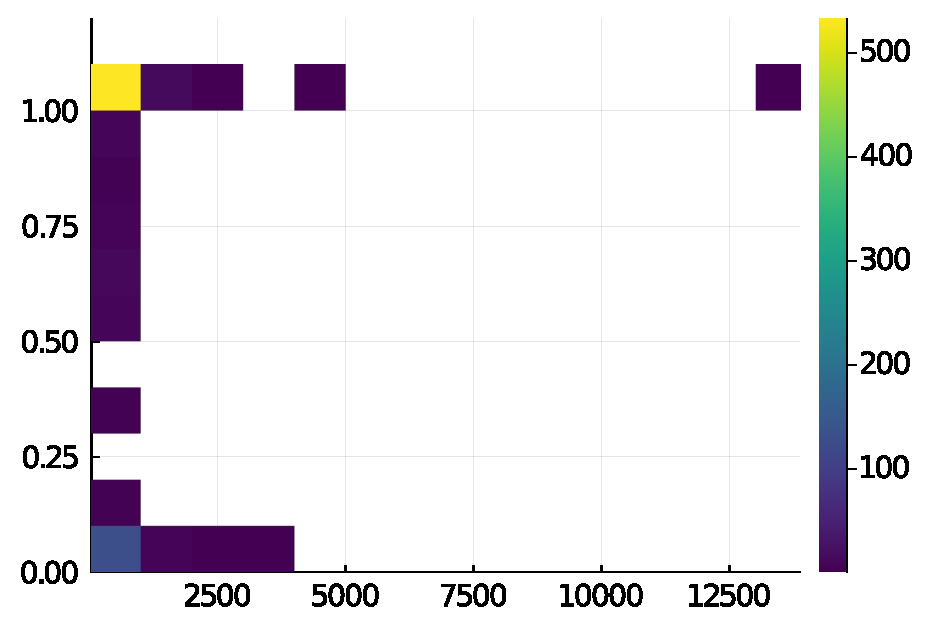
\includegraphics[width=\textwidth]{figs/Pluto-size-vs-stable.pdf}
     \end{subfigure}
     \ \ \
     \begin{subfigure}[b]{0.35\textwidth}
       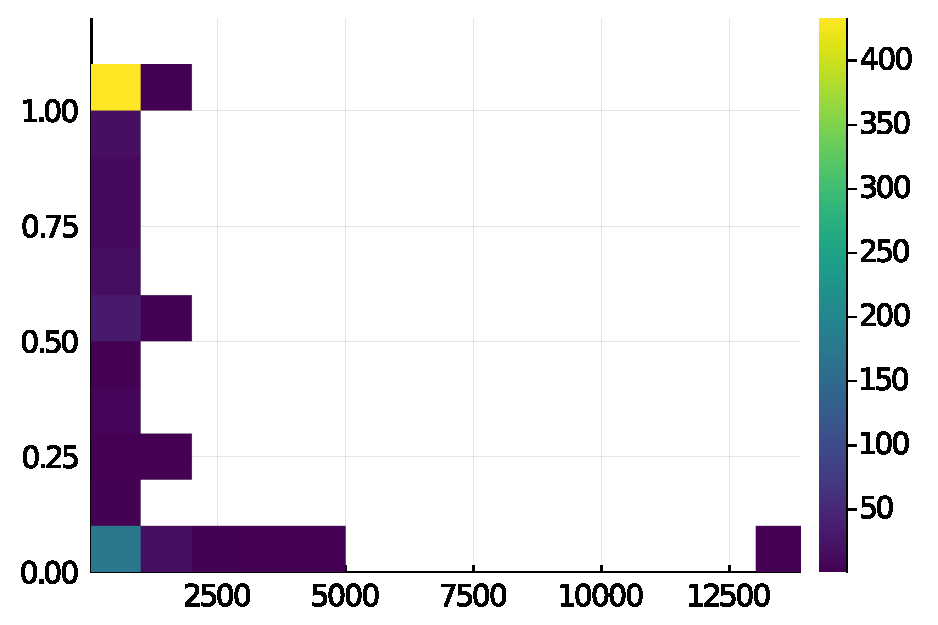
\includegraphics[width=\textwidth]{figs/Pluto-size-vs-grounded.pdf}
     \end{subfigure}
\caption{Stability (left, OY axis) and groundedness (right, OY) by method size (OX) in Pluto}%
\label{figs:size:Pluto:main}
\end{figure}

The graphs for all of the 10 packages listed in
Table~\ref{empirical:fig:top} are genertaed for all combinations of the properties of
interest\PAPERVERSIONINLINE{~\cite{oopsla21jules:arx}}{; the graphs are provided in \appref{sec:app}}.
Most of the graphs look very similar to the ones from
Fig.~\ref{figs:size:Pluto:main}, which depicts Pluto---a package for creating
Jupyter-\hspace{0pt}like notebooks in Julia. In the following paragraphs, we
discuss features of these graphs and highlight the discrepancies.

The first distinctive feature of the graphs is the hot area in the top-left
corner: most of the 10 packages employ many small, stable/grounded methods;
the bottom-left corner is usually the second-most hot, so a significant number
of small methods are unstable/ungrounded. For the Knet package,
these two corners are reversed; for DifferentialEquations, they are reversed
only on the groundedness plot. Both of these facts are not surprising after seeing
Table~\ref{empirical:fig:top}, but having a visual tool to discover such facts
may be useful for package developers.

The second distinctive feature of these graphs is the behavior of large,
ungrounded methods (bottom-right part of the right-hand-side graph). The
``tail'' of large methods on the groundedness graphs almost always lies below
the $1$-level; furthermore, larger methods tend to be less grounded.
However, if we switch from groundedness to stability plots, a large portion of
the tail jumps to the $1$-level. This means larger methods are unlikely to be
grounded (as expected, because of the growing number of registers), but they
still can be stable and thus efficiently used by other methods. Pluto provides a
good example of such a method: its \c{explore!} method of size 13003 (right-most
rectangle on Fig.~\ref{figs:size:Pluto:main}, 330 lines in the source code) analyzes
Julia syntax trees for scope information with a massive \c{if/else if/..} statement.
This method has a very low chance of being grounded, and it was not grounded on the
runs I analyzed. However, the method has a concrete return type annotation, so
Julia (and the programmer) can easily see that it is stable.

% %% PLZ, DO NOT DELETE THIS
% % Plots where the size axis is replaced with the number of branching or return
% % instructions have a technical difference from what we see on
% % Fig.~\ref{figs:size:Pluto:main} in that they reflect individual method instances
% % instead of methods because due to Julia's simple optimizer, which kicks i
% % when the main optimizer is turned off by our demand, instances of a method can
% % have different number of those instructions. As a consequence, all squares on
% % the histograms lie either on $1$-level or $0$-level. Otherwise, the picture is
% % similar to Fig.~\ref{figs:size:Pluto:main} in the two distinctive feature discussed
% % above.

% In the case of the number of gotos and returns, the plots are largely similar
% to the ones for method size, but they highlight one more package with low
% groundedness. Namely, the Gen package (aimed at probabilistic
% inference~\cite{JuliaGenPkgPub2019}) has the hottest area in the bottom-left
% corner, contrary to the first general property we identified for the size-based
% plots. Recall (Tables \ref{empirical:fig:all} and \ref{empirical:fig:top}) that
% Gen's groundedness is 14\% less than the average on the whole corpus of
% \goodpkgsnum packages.

\paragraph{Manual Inspection}

To better understand the space of stable methods,
I perform a qualitative analysis of a sample of stable methods that
have either large sizes or many instances.

Many large methods have one common
feature: they often have a return type ascription on the method header of
the form:
\begin{lstlisting}[language=julia]
function f(...) :: Int
  ...
end
\end{lstlisting}
These ascriptions are a relatively new tool in Julia, and they are used only
occasionally, in our experience. An ascription makes the Julia compiler insert implicit
conversions on all return paths of the method. Conversions are user extendable:
if the user defines type \c{A}, they can also add methods of a special
function \c{convert} for conversion to \c{A}. This function will be called
when the compiler expects \c{A} but infers a different type, for example,
if the method returns \c{B}.
If the method returns \c{A}, however, then \c{convert} is a no-op.

Type ascriptions may be added simply as documentation, but they can also
be used to turn type instability into a run-time error:
if the ascribed type is concrete and a necessary conversion is not available,
the method will fail. This provides a useful, if
unexpected, way to assure that a large method never becomes unstable.

While about 85\% of type-stable methods in the top 10 packages are uninteresting
in that they always return the same type, sampling the rest illuminates
a clear pattern: the methods resemble what we
are used to see in statically typed languages with parametric polymorphism.
% Below is a list of categories that we identify in this family.
Here are the subcategories identified in this group of methods.

\begin{itemize}
\item
  Various forms of the identity function---a surprisingly popular function that
  packages keep reinventing. In an impure language, such as Julia, an identity
  function can produce various side effects.
  For example, the Genie package adds a caching effect to
  its variant of the identity function called \c{secret_token!}.

\item Container manipulations for various kinds of containers, such as arrays,
  trees, or tuples. For instance, the Flux package defines the
  \c{extraChain} function that maps a tuple of functions by applying
  them to a given argument.

\item
  Smart constructors for user-defined polymorphic structures. For example, the
  \c{build_constraint} convenience function from JuMP creates an instance of the
  \c{VectorConstraint} structure with three fields, each of which is polymorphic.

\item
  Type computations---an unusually wide category for a dynamically typed
  language. For instance, the Gen package defines a type that represents generative
  functions in probabilistic programming; the type has two type parameters, for
  argument and for return type of the function; in order to extract those type
  arguments (and return them as objects) Gen defines two simple polymorphic functions.

\end{itemize}

\subsection{Main Results}

My analysis shows that a Julia user can expect mostly stable (74\%) and
somewhat grounded (57\%) code in widely used Julia packages. If the authors
are intentional about performance and stability, as demonstrated by the Genie
package, those numbers can be much higher. Although my sample of packages is
too small to draw strong conclusions, several factors can be
used by a Julia programmer to pinpoint potential sources of instability in their
package. For example, in some cases, varargs methods might indicate instability.
Large methods, especially ones with heavy control flow,
tend to not be type grounded but often are stable; in particular,
if they always return the same concrete type.
Finally, although highly polymorphic methods are neither stable nor unstable
in general, code written in the style of parametric polymorphism
often suggests type stability.

My dynamic analysis and visualization code is written in Julia (and some bash
code), and relies on the vanilla Julia implementation. Thus, it can be employed
by package developers to study type instability in their code, as well as check
for regressions.


\section{Formalizing Type Stability: Jules}%
\label{sec:jules}


Formal reasoning about type stability and groundedness is based on
\jules, an abstract machine that provides an idealized version of
Julia's intermediate representation (IR) and compilation model.
\jules captures the just-in-time (JIT) compilation process that (1) specializes methods
for concrete argument types as the program executes, and (2) replaces dynamically
dispatched calls with direct method invocations when \emph{type inference}
is able to get precise information about the argument types.
% Note that type inference algorithm directly affects
% type stability and groundedness of code, and thus the ability of the JIT compiler
% to optimize it. While Julia's actual type inference algorithm
% is quite complex, its implementation is not relevant for understanding
% our properties of interest; thus, \jules abstracts over type inference
% and uses it as a black box.

\begin{figure}[!h]
  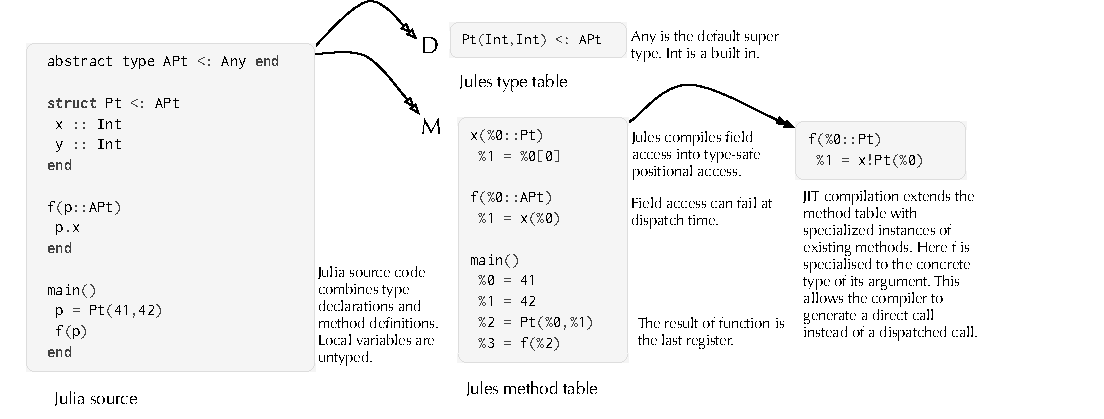
\includegraphics[width=1.1\columnwidth]{figs/compile.pdf}
  \caption{Compilation from Julia to \jules}\label{comp}
\end{figure}

Fig.~\ref{comp} illustrates the relationship between Julia source code, the
\jules intermediate representation, and the result of compilation. I do not model
the translation from the source to \jules, and simply assume that the front-end
generates well-formed \jules code.\footnote{The front-end does not devirtualize
function calls, as Julia programmers do not have the ability to write direct
method invocations in the source.} A \jules program consists of an immutable \emph{type
table}~\tytbl and a \emph{method table}~\mtbl; the method table can be incrementally extended
with method instances that are compiled by the just-in-time compiler.

The source program of Fig.~\ref{comp} defines two types, the concrete \c{Pt} and
its parent, the abstract type \c{APt}, as well as two methods, \c{f} and
\c{main}. When translated to \jules, \c{Pt} is added to the type table along
with its supertype \c{APt}. Similarly, the methods \c{main} and \c{f} are added
to the \jules method table, along with accessors for the fields of \c{Pt}, with
bodies translated to the \jules intermediate representation.

The \jules IR is similar to static single assignment form. Each statement can
access values in registers, and saves its result into a new, consecutively
numbered, register. Statements can perform a dispatched call \c{f(\%2)}, direct
call \c{x\!Pt(\%0)}, conditional assignment (not shown), and a number of other
operations. The IR is untyped, but the translation from Julia is type sound. In
particular, type soundness guarantees that only dispatch errors can occur at run
time. For example, compilation will produce only well-formed field accesses such
as the one in \c{x(\%0::Pt)}, but a dispatched call \c{x(\%0)} in \c{f} could
fail if \c{f} was called with a struct that did not have an \c{x} field. In
order to perform this translation, \jules uses type inference to determine the
types of the program's registers. I abstract over this type inference mechanism
and only specify that it produces sound (with respect to our dynamic semantics)
results. %, but do not describe its operation.

Execution in \jules occurs between \emph{configurations} consisting of both
a stack of \emph{frames} \frm (representing the current execution state)
and a \emph{method table} \mtbl (consisting of original methods and specialized
instances), denoted $\config{\frm}{\mtbl}$. A configuration
$\config{\frm}{\mtbl}$ evolves to a new configuration
$\config{\frm'}{\mtbl'}$ by stepping $\config\frm\mtbl \step
\config{\frm'}{\mtbl'}$; every step processes the top instruction in $\frm$
and possibly compiles new method instances into $\mtbl'$.
% Notably, due to the
% so-called world-age mechanism~\cite{oopsla20a} which restricts the effect
% of \c{eval}, source methods are fixed from the
% perspective of compilation; only compiled instances changes.

\subsection{Syntax}

The syntax of \jules methods is defined in~\figref{syntax}.
There are two key
notational devices. First, sequences are denoted \ol{\,\cdot\,}; thus, \ol\ty
stands for types $\ty_0\dots\ty_n$, \ol{\v\k} for registers $\v\k_0\dots\v\k_n$,
and \ol\st for instructions $\st_0\dots\st_n$. An empty sequence is written
\emp. Second, indexing is denoted $[\cdot]$; \idx{\ol\ty}\k is the $k$-th type
in \ol\ty (starting from 0), \get\j\k is the $k$-th field of \v\j, and
\idx\mtbl{\msig\m{\ol\ty}} indexes \mtbl by method signature where \m denotes
method name and \ol\ty denotes argument types.

\begin{figure}[!h]\footnotesize
% \begin{tabular}{lcl}
\begin{tabular}{lll}
\ty &::=& \Ty  \\
    & | & \aty \\
\\
  \tytbl &::=& $\left(\ \ \msig\Ty{\ol\ty} ~<:~ \aty \ \ \right)\!*$
\\
\\
  \mtbl  &::=& $\left(\ \ \langle \meth\m{\ol{\ty'}}{\ol{\v\j}}\ol\st,\ \ol{\ty}\rangle \ \ \right)\!*$
\\
\end{tabular}
% &\;&
~%
\begin{tabular}{ll@{~}ll}
\st &::=& & instruction\\
    & | & $\ass\i\p$                                       &\it int. assignment\\
    & | & $\ass\i{\v\j}$                                   &\it reg. transfer\\
    & | & $\ass\i{\construct\Ty{\ol{\v\k}}}$               &\it allocation\\
    & | & $\ass\i{\get\j\k}$                               &\it field access\\
    & | & $\cond\i\j{\call\m{\ol{\v\k}}}{\v\l}$            &\it dispatched call\\
    & | & $\cond\i\j{\direct\m{\ol{\Ty}}{\ol{\v\k}}}{\v\l}$&\it direct call\\
    & \multicolumn{2}{l}{$i \in \mathbb{N},\ \p \in \mathbb{Z}$}                 &  \\
\end{tabular}
% \end{tabular}
\caption{Syntax of \jules}\label{syntax}
\end{figure}

Types \ty live in the immutable type table \tytbl, which contains both concrete
(\Ty) and abstract (\aty) types. Each type table entry is of the form
$\msig{\Ty}{\ol\ty} <: \aty$, introducing concrete type $\Ty$, with fields of
types $\ol\ty$, along with the single supertype $\aty$. Two predefined types are
the concrete integer type \int, and the universal abstract supertype \any.

Method tables \mtbl contain method definitions of two sorts:
first, original methods that come from source code;
second, method instances compiled from original methods.
To distinguish between the two sorts, \jules stores the type signature of the
original method in every table entry.
Thus, table entry
$\langle\meth\m{\ol{\ty'}}{\ol{\v\j}}\ol\st,\ \ol{\ty}\rangle$ describes a
method \m with parameter types $\ol{\ty'}$ and the body comprised of
instructions $\ol\st$; type signature \ol{\ty} points to the original method.
If \ol\ty is equal to \ol{\ty'}, the entry defines an original method,
and \ol{\st} cannot contain direct calls.
Otherwise, \ol{\ty'}
denotes some concrete types~\ol\Ty, and the entry defines a
method instance compiled from \msig\m{\ol\ty}, specialized for concrete argument
types $\ol\Ty <: \ol\ty$.
Method table may contain multiple method definitions with the same name,
but they have to have distinct type signatures.

Method bodies consist of instructions \ol{\st}. An instruction $\v{\i}
\leftarrow \text{\c{op}}$ consists of an operation \c{op} whose result is
assigned to register $\v\i$. An instruction can assign from a primitive integer
\p, another register \v\j, a newly created struct $\construct\Ty{\ol{\v\k}}$
of type \Ty with field values $\ol{\v\k}$, or the result of looking up a struct
field as $\get\j\k$. Finally, the instruction may perform a function call. Calls
can be dispatched, $\call\m{\ol{\v\k}}$, where the target method is dynamically
looked up, or they can be direct, \direct\m{\ol\Ty}{\ol{\v\k}}, where the target
method is specified. All calls are conditional: \EM{\v\j ~?~ \text{\c{call}} :
  \v\l}, to allow for recursive functions.
If the register \v\j is non-zero, then \c{call} is performed. Otherwise,
the result is the value of register \v\l. Conditional calls can be trivially
transformed into unconditional calls; in examples, this transformation is
performed implicitly.

\subsection{Dynamic Semantics}

\jules is parameterized over three components: method dispatch $\mathcal D$,
type inference $\mathcal I$, and just-in-time compilation \jit. I do not
specify how the first two work, and merely provide their interface and a set of
criteria that they must meet (in sections \ref{sec:disp} and \ref{sec:infer},
respectively). The compiler, \jit, is instantiated with either the identity
function, which gives a regular non-optimizing semantics, or an optimizing
compiler, which is defined in section~\ref{sec:comp}. The optimizing compiler
relies on type inference $\mathcal I$ to devirtualize method calls. Type
inference also ensures well-formedness of method tables. Method dispatch
$\mathcal D$ is used in operational semantics.

\begin{figure}[!t]\small
\begin{tabular}{rclcrclcrcl}
\val &::=& \p\ |\ \construct\Ty{\ol\val}
& \qquad &
\env &::=& \ol\val
& \qquad &
\frm &::=& \done\ |\ \stk{\env\ \ol\st}{\frm} \\
\end{tabular}
\begin{mathpar}
\PAPERVERSIONINLINE{}{\framebox{\configd \step \config{\frm'}{\mtbl}}\\}

\inferrule[Prim]{
  \st = \ass\i\p\\\\
  \env' = \env + \p
}{
  \config{ \stk{ \env \ \st\,\ol\st}{\frm} }{\mtbl} \step
  \config{ \stk{ \env'\ \ol\st     }{\frm} }{\mtbl}
}

\inferrule[Reg]{
  \st = \ass\i{\v\j}\\\\
   \env'=\env + \idx\env\j
}{
  \config{ \stk{ \env \ \st\,\ol\st}{\frm} }{\mtbl} \step
  \config{ \stk{ \env'\ \ol\st     }{\frm} }{\mtbl}
}

\inferrule[New]{
  \st= \ass\i{\construct\Ty{\ol{\v\k}}}\\\\
  \env'  = \env + \construct\Ty{\idx\env{\ol{k}}}
}{
  \config{ \stk{ \env \ \st\,\ol\st }{\frm} }{\mtbl} \step
  \config{ \stk{ \env'\ \ol\st      }{\frm} }{\mtbl}
}
\\

\inferrule[Field]{
  \st= \ass\i{\get\j\k}\\\\
  \val = \idx\env\j \and
  \env' = \env + \idx\val\k
}{
  \config{ \stk{ \env \ \st\,\ol\st }{\frm} }{\mtbl} \step
  \config{ \stk{ \env'\ \ol\st      }{\frm} }{\mtbl}
}

\inferrule[False1]{
  \st= \cond\i\j{\call\m{\ol{\v k}}}{\v\l}\\\\
  0 = \idx\env\j \and
  \env'=\env +  \idx\env\l
}{
  \config{ \stk{ \env \ \st\,\ol\st }{\frm} }{\mtbl} \step
  \config{ \stk{ \env'\ \ol\st      }{\frm} }{\mtbl}
}

\inferrule[False2]{
  \st= \cond\i\j{\direct\m{\ol\Ty}{\ol{\v\k}}}{\v\l}\\\\
  0 = \idx\env\j \and
  \env'=\env + \idx\env\l
}{
  \config{ \stk{ \env \ \st\,\ol\st }{\frm} }{\mtbl} \step
  \config{ \stk{ \env'\ \ol\st      }{\frm} }{\mtbl}
}
\\

\inferrule[Disp]{
  \st= \cond\i\j{\call\m{\ol{\v\k}}}{\v\l}\\\\
  0 \not=\idx\env\j \and
  \ol\Ty = \typeof(\idx\env{\ol{k}}) \and
  \mtbl' = \jit(\mtbl, \m, \ol\Ty) \\\\\
  \ol{\st'} = \body(\dispatch{\mtbl'}\m{\ol\Ty}) \and
  \env' =  \idx\env{\ol{k}}
}{
  \config{                        \stk{\env\ \st\,\ol\st}{\frm}  }{\mtbl} \step
  \config{ \env'\ \stk{\ol{\st'}}{\stk{\env\ \st\,\ol\st}{\frm}} }{\mtbl'}
}

\inferrule[Direct]{
  \st= \cond\i\j{\direct\m{\ol\Ty}{\ol{\v\k}}}{\v\l}\\\\
  0 \not = \idx\env\j \\\\
  \ol{\st'} = \body(\mtbl[\msig\m{\ol\Ty}]) \and
  \env' = \idx\env{\ol{k}}
}{
  \config{                        \stk{\env\ \st\,\ol\st}{\frm}  }{\mtbl} \step
  \config{ \env'\ \stk{\ol{\st'}}{\stk{\env\ \st\,\ol\st}{\frm}} }{\mtbl}
}

\inferrule[Ret]{
  \env''=\env + \last{\env'}
}{
  \config{ \stk{\env'\ \done}{\stk{ \env  \ \st\,\ol\st }{\frm}}}{\mtbl} \step
  \config{                    \stk{ \env''\ \ol\st      }{\frm} }{\mtbl}
}
\end{mathpar}
\caption{Operational semantics of Jules}\label{sems}
\end{figure}

\paragraph{Operational Semantics}\label{sec:opsem}

Fig.~\ref{sems} gives rules for the dynamic semantics. Given a type table \tytbl
as context, \jules can step a configuration $\config{\frm}{\mtbl}$ to
$\config{\frm'}{\mtbl'}$, written as $\config\frm\mtbl \step
\config{\frm'}{\mtbl'}$.
Stack frames \frm consist of a sequence of environment-instruction list pairs.
Thus, $\stk{\env\ \ol\st}\frm$ denotes a stack with environment \env and
instructions \ol\st on top, followed by a sequence of environment-instruction
pairs. Each environment is a list of values $\env=\ol\val$, representing
contents of the sequentially numbered registers. Environments can then be
extended as $\env + \val$, indexed as $\idx\env\k$, and their last value is
\last\env if \env is not empty.

% The small-step dynamic semantics is largely straightforward. The first four
% rules deal with register assignment: updating the environment with a constant
% value (\SC{Prim}), the value in another register (\SC{Reg}),
% a newly constructed struct (\SC{New}), or the value in a field (\SC{Field}).
% The remaining five rules deal with function calls, either dispatched
% \call\m{\ol{\v\k}} or direct \direct\m{\ol\Ty}{\ol{\v\k}}.
% Call instructions are combined with conditioning: a call can only be made after
% testing the register \v\j, called a guard register.
% If the register value is zero, then the value of the alternate register
% \v\l is returned (\SC{False1/False2}).
% Otherwise, the call can proceed, by \SC{Disp} for dispatched calls and \SC{Direct}
% for direct ones.
% %
The most interesting rule in the semantics is the one representing dispatched
calls (\SC{Disp}). A dispatched call starts by prompting the JIT compiler to
specialize method \m from the method table~\mtbl with the argument types \ol\Ty
and produce a new method table $\mtbl'$. Next, using the new table $\mtbl'$, the
dispatch mechanism $\mathcal D$ determines the method to invoke. Finally, the
body \ol{\st'} of the method and call arguments \idx\env{\ol{k}} form a new
stack frame for the callee, and the program steps with the extended stack and
the new table.
% %
% Direct calls are simpler because
% a direct call $\msig\m{\ol\Ty}$ uniquely identifies the
% method to invoke. Thus, the method's instructions are looked up in \mtbl
% by the method signature, a new stack frame is created,
% and the program steps with the new stack and the same method table.
% %
% The top frame without instructions to execute indicates the
% end of a function call (\SC{Ret}): the last value of the top-frame environment
% becomes the return value of the call, and the top frame is popped from the stack.

% Program execution begins with the frame $\emp\ \main()$%
% \footnote{Recall that unconditional calls are implicitly expanded into conditional ones.},
% i.e. a call to the \main function with an empty environment;
% the execution either diverges, finishes with a final configuration $\env\ \done$,
% or runs into an error.
% We define two notions of error. An \emph{err} occurs only in the \SC{Disp} rule,
% when the dispatch function $\mathcal D$ is undefined for the call; the \emph{err}
% corresponds to a dynamic-dispatch error in Julia. A configuration is
% \emph{wrong} if it cannot make a step for any other reason.
% %the program is ill-formed. while \emph{erred} states are merely ill-typed.
% %JB: we don't define a type system, so I would not use "ill-typed" terminology

% \begin{definition}[Errors] A non-empty configuration \frm, \mtbl
%  that cannot step $\frm, \mtbl \step \frm', \mtbl'$ has \emph{erred} if its
%  top-most frame, \E\ \ol\st, starts with $\cond\i\j{\call\m{\ol{\v\k}}}{\v\l}$,
%  where \ol\Ty is the types of \ol{\v\k} in \E, $\m\in\mtbl$, and
%  \dispatch\mtbl\m{\ol\Ty} is undefined. Otherwise, \frm, \mtbl is
%  \emph{wrong}.
% \end{definition}


\paragraph{Dispatch}\label{sec:disp}

\jules is parametric over method dispatch: any mechanism $\mathcal D$ that
satisfies a technical requirement called \emph{Dispatch Contract} can be used.
For instance, Julia's dispatch mechanism, given method table, method name, and argument types,
returns the \emph{most specific method applicable} to the given arguments
if such a method exists and is unique. This means: first, applicable
methods are those whose declared type signature is a supertype of the argument
type; second, the most specific method is the one whose type signature is the
most precise; third, only one most specific applicable method may exist, or
else an error is produced. Each of these components appear in our technical
requirement mentioned above. Note that the first two notions require subtyping
decision procedure available~--- a challenge on its own~\cite{oopsla18b}. Abstracting over
$\mathcal D$ avoids this irrelevant complication.

% \begin{definition}[Dispatch Contract] The \emph{dispatch} function
%   $\dispatch\mtbl\m{\ol\Ty}$ takes method table \mtbl, method name \m,
%   and concrete argument types \ol\Ty, and returns a method
%   $\meth\m{\ol{\ty}}{\ol{\v\j}}\ol\st \in \mtbl$ such that
%   the following holds (we write $\ol\ty <: \ol{\ty'}$ as a shorthand for
%   $\forall i.\,\ty_i<:\ty'_i$):
%   \begin{enumerate}
%     \item $\ol\Ty <: \ol\ty$, meaning that $\msig\m{\ol\ty}$
%       is applicable to the given arguments;
%     \item $\forall \meth\m{\ol{\ty'}}{\ol{\v\j}}\ol\st \in \mtbl.\ \
%       \ol\Ty <: \ol{\ty'}\ \implies\ \ol{\ty} <: \ol{\ty'},$
%       meaning that $\msig\m{\ol\ty}$ is the most specific applicable method.
%   \end{enumerate}
%   \label{disprel}
% \end{definition}

\paragraph{Inference}\label{sec:infer}

The Julia compiler infers types of variables by forward data-flow analysis. Like
dispatch, inference is complex, so I parameterize over it. For our purposes, an
inference algorithm~$\mathcal I$ returns a sound typing for a sequence of
instructions in a given method table,
$\typeinf{\origmtbl{\mtbl}}{\ol\ty}{\ol\st}=\ol{\ty'}$, where \origmtbl{\mtbl}
denotes the table containing only methods without direct calls. Inference
returns types $\ol\ty'$ such that each $\ty'_i$ is the type of register of
$\st_i$. Any inference algorithm that satisfies two technical requirements, soundness and
monotonicity, is acceptable.

\paragraph{Compilation}\label{sec:comp}
%
Devirtualization in \jules happens when the \SC{Disp} rule invokes the
$\jit(\mtbl,\m,\ol\Ty)$ relation. The relation specializes methods according to
the inferred type information, replacing
% non-\emph{err}
dispatched calls with direct calls where
possible. In particular, dispatched calls
cause a recursive JIT invocation, followed by rewriting to a direct call. To
avoid recursive compilation, a stub method $\langle \msig\m{\ol{\Ty}}\done,
\ol\ty \rangle$ is added at the beginning of compilation,
and over-written when compilation is done. As the source program is finite and
new types are not added during compilation, it terminates.


\subsection{Main Results}%
\label{sec:stability-formal}\label{sec:jit-correct}

Using the formalization shown above, I define type stability and type
groundedness in \jules and prove the following.

\begin{itemize}
  \item
Type stability is a necessary (but not sufficient)
condition for type groundedness.

  \item
Type-grounded methods
compile to method instances without dynamically dispatched calls.

  \item
The compiler is correct: if the \jit relation is replaced by the one that
does nothing, the result of evaluation of the program remains the same.
\end{itemize}

% \begin{definition}[Stable and Grounded]\label{def:ground}
%   Let \meth{\m}{\ol\ty}{}{\ol\st} be an original method in a well-formed
%   method table \mtbl. Given concrete argument types $\ol\Ty <: \ol\ty$,
%   if $\typeinf{\origmtbl{\mtbl}}{\m}{\ol\Ty} = \ol{\ty'}$,
%   and
%   \begin{enumerate}
%   \item  $\last{\ol{\ty'}} = \Ty'$, i.e. the return type is concrete, then
%     the method is \emph{type stable for \ol\Ty},
%   \item $\ol{\ty'} = \ol{\Ty'}$, i.e. all register types are concrete, then the
%     method is \emph{type-grounded for \ol\Ty}.
%   \end{enumerate}

%   Furthermore, a method is called \emph{type stable (grounded) for a set $W$
%   of concrete argument types} if it is type stable (grounded) for every
%   $\ol\Ty \in W$.
% \end{definition}



% ****************************************************************************************
%              Chap. 4: Plan of Work
% ****************************************************************************************


\chapter{Plan of Work}%
\label{chap-plan}

The remaining work is the third task of those declared in
\secref{chap-problem} (Research Problem): an approach to
approximate type stability statically, without running
the compiler. I am currently working on this task and have a draft of this
approach, as well as a tool implementing it.
The tool successfully runs on several sample packages but the output needs to be
validated.
I plan to analyze the data, augment the approach if necessary, and
write up the results as a paper to be submitted for
OOPSLA '23. After that I will write the dissertation, which
should take until March 2023. I intend to defend the thesis in April 2023 (the
end of Spring semester at Northeastern).

\begin{center}
  \begin{tabular}{ll}
    \toprule
    \textbf{Month} & \textbf{Task} \\
    \midrule
    June-October & Approximating Type Stability\\
    October & OOPSLA '23 Submission\\
    November---March & Dissertation\\
    April & Defense\\
    \bottomrule
  \end{tabular}
\end{center}


% ****************************************************************************************
%              Bibliography
% ****************************************************************************************


% work-around to have small caps also here in the headline
% https://tex.stackexchange.com/questions/188126/wrong-header-in-bibliography-classicthesis
% Thanks to Enrico Gregorio
\defbibheading{bibintoc}[\bibname]{%
  \phantomsection
  \manualmark
  \markboth{\spacedlowsmallcaps{#1}}{\spacedlowsmallcaps{#1}}%
  \addtocontents{toc}{\protect\vspace{\beforebibskip}}%
  \addcontentsline{toc}{chapter}{\tocEntry{#1}}%
  \chapter*{#1}%
}
% newpage starts bibliography from a newpage and increments page number in
% contents section
\newpage
\printbibliography[heading=bibintoc]

\end{document}

\endinput{}
